\documentclass[a4paper,12pt, openany]{book}  % Book class for thesis 
\usepackage[utf8]{inputenc}
\usepackage{graphicx}
\usepackage{geometry}
\geometry{left=2cm, right=2cm, top=2cm, bottom=2cm} 
\usepackage{setspace}
\setstretch{1}
\raggedbottom
\usepackage{titlesec}
\usepackage[toc,page]{appendix}
\titleformat{\subsection}[hang]{\normalfont\large\bfseries}{\thesubsection}{1em}{}
\titlespacing*{\subsection}{0pt}{\baselineskip}{0.5\baselineskip}
\usepackage[bottom]{footmisc}
\usepackage{ragged2e}
\usepackage{ltablex}
\keepXColumns
\renewcommand\tabularxcolumn[1]{>{\noindent\justifying\arraybackslash}m{#1}}

\usepackage{amssymb}
\usepackage{pifont}%
\newcommand{\cmark}{\ding{51}}%
\newcommand{\xmark}{\ding{55}}%
\usepackage{lmodern}
\usepackage{fancyhdr}
\usepackage{tocloft}
\usepackage{xcolor}
\usepackage[
    colorlinks=true,        % disables boxes around links
    urlcolor=teal,          % URL link color
    linkcolor=black,        % color of internal links (e.g., TOC)
    citecolor=blue
]{hyperref}
\usepackage[nameinlink,noabbrev]{cleveref}
\usepackage{array}
\usepackage[nottoc]{tocbibind}
\usepackage{booktabs}
\usepackage{float}
\usepackage[T1]{fontenc}
\usepackage{soul}  
\usepackage[font=bf,labelfont=bf,justification=raggedright,singlelinecheck=false]{caption}

\captionsetup{font={bf,small}, labelfont=bf, justification=raggedright, singlelinecheck=false}

\usepackage{chngcntr}
\counterwithout{footnote}{chapter}
\counterwithout{figure}{chapter}
\counterwithout{table}{chapter}

\usepackage{amssymb}
\usepackage{fvextra}
\usepackage{listings}
\lstset{
  breaklines=true,
  basicstyle=\ttfamily\small,
  frame=single
}

\usepackage{multirow, tabularx, xurl}

\usepackage[authordate,backend=biber,natbib]{biblatex-chicago}
\ExecuteBibliographyOptions{maxcitenames=2, mincitenames=1}
\DeclareDelimFormat{nameyeardelim}{\addcomma\space}
\addbibresource{references.bib}
\AtEveryCitekey{%
  \ifciteseen
    {}
    {\color{blue}}%
}
\renewbibmacro*{doi+eprint+url}{
  \printfield{doi}
}
\DeclareCiteCommand{\citep}
  {\begingroup(}  % Start a group, manually insert black opening parenthesis
  {\color{blue}\usebibmacro{citeindex}%
   \usebibmacro{cite}}
  {\multicitedelim}
  {\usebibmacro{postnote}\endgroup)}  % Close blue group, then black parenthesis
\DeclareFieldFormat{doi}{%
  DOI: \ifhyperref
    {\href{https://doi.org/#1}{#1}}
    {#1}}

% Page numbering setup (BOTTOM CENTER)
\pagestyle{fancy}
\fancyhf{} % Clear all headers and footers
\renewcommand{\headrulewidth}{0pt} % Remove header line
\fancyfoot[C]{\thepage} % Center page number in footer

% Apply same style to chapter start pages
\fancypagestyle{plain}{%
  \fancyhf{}
  \renewcommand{\headrulewidth}{0pt}
  \fancyfoot[C]{\thepage}
}

% Chapter formatting
\titleformat{\chapter}[display]
  {\normalfont\huge\bfseries}
  {\chaptertitlename\ \thechapter}{20pt}{\Huge} 

\titlespacing*{\subsubsection}{2em}{*0}{*0}


% Customize Table of Contents
\setlength{\cftbeforetoctitleskip}{-1em} % Reduce space before title
\setlength{\cftaftertoctitleskip}{1.5em} % Space after title
\setlength{\cftbeforetoctitleskip}{50pt} % Space above TOC title (same as chapters)
\renewcommand{\cftchappagefont}{\normalfont} % Page numbers normal
\renewcommand{\cftchapdotsep}{\cftdotsep} % Add dot leaders
\setlength{\cftbeforesecskip}{0.5ex} % Reduce space between sections
% Add List of Figures/Tables to TOC
\renewcommand{\listfigurename}{List of Figures}
\renewcommand{\listtablename}{List of Tables}

\usepackage{pdfcomment}
\begin{document}

% Frontispiece
\begin{titlepage}
    \centering
    
\includegraphics[width=0.2\textwidth]{images/unibo-logo.pdf}
    
    \vspace*{1cm}
    \Large
    \textbf{ALMA MATER STUDIORUM \\ 
    UNIVERSITÀ DI BOLOGNA}
    
    
    \vspace{1.5cm}
    
    \normalsize
    \textsc{Department of Classical Philology and Italian Studies} \\
    \vspace{0.5cm}
    \textsc{Second Cycle Degree in} \\
    \vspace{0.2cm}
    \textsc{\textbf{Digital Humanities and Digital Knowledge}}
    
    \vspace{1.6cm}
    
    \begin{spacing}{1}
    \LARGE
    \textbf{From Documents to Dialogue:\\Design, Implementation and Evaluation of a Question-Answering System for Geoportale Nazionale Archeologia}
    \end{spacing}
    
    \vspace{1.2cm}
    \normalsize
    Dissertation in\\
    \textbf{Machine Learning for the Arts and Humanities}
    
    \vspace{1cm}
    
    \begin{tabbing}
    \textbf{Supervisor} \hspace{10cm} \= \textbf{Defended by} \\
    Prof. Giovanni Colavizza \> Lucrezia Pograri \\
    \\
    \textbf{Co-Supervisors}\\
    Prof. Paolo Bonora \\
    Mario Caruso and Simone Persiani, BUP Solutions
    \end{tabbing}
    
    \vfill
    \rule{\linewidth}{0.4pt}
    \vspace{0.2cm}
    
    \textbf{Graduation Session II} \\
    \textbf{Academic Year 2024/2025}
    
\end{titlepage}
\newpage
\thispagestyle{empty}  % Force blank page to have no header/footer
\mbox{}                % Prevent "empty page" warning
\setcounter{figure}{0}

%\pagestyle{empty}
% Front Matter (Roman page numbering)
\frontmatter
\pagestyle{fancy}
\tableofcontents

% Abstract
\chapter{Abstract}
\label{chap:abstract}
\pdfcomment{WIP}
\begin{spacing}{1.5}
This dissertation presents the design and development of a question-answering (QA) system tailored to the Geoportale Nazionale Archeologia (GNA). The research addresses the challenge of extracting relevant information from archaeological documentation using Retrieval-augmented generation (RAG) amd natural language processing (NLP) techniques. The methodology combines transformer-based language models with domain-specific information extraction to enable intuitive, natural language querying of technical documentation related to archaeological data.

% Key findings demonstrate significant improvements in retrieval accuracy compared to traditional search methods, with a 25\% increase in F1-score. 

% conclusion

\vspace{\baselineskip} % Add vertical space before keywords
\noindent\textbf{Keywords:} Digital Humanities \textperiodcentered\ Information Retrieval \textperiodcentered\ Question-Answering Systems \textperiodcentered\ Retrieval-Augmented Generation \textperiodcentered\ Natural Language Processing \textperiodcentered\ AI \textperiodcentered\ Cultural Heritage.

\end{spacing}
\clearpage
\listoffigures
\clearpage
\listoftables

\newpage
\thispagestyle{empty} 
\mbox{}                

% Main Content (Arabic page numbering)
\mainmatter
\pagestyle{fancy}
\renewcommand{\figureautorefname}{Fig.}
\renewcommand{\tableautorefname}{Tab.}
\renewcommand{\chapterautorefname}{Chap.}
\renewcommand{\sectionautorefname}{Sec.}
\makeatletter
\renewcommand{\thefootnote}{\textsuperscript{\arabic{footnote}}}
\renewcommand\@makefntext[1]{%
  \noindent
  \parindent=0pt
  \leftskip=0pt
  \hb@xt@1.8em{\hss\@thefnmark}#1%
}
\makeatother

\chapter{Introduction}
\label{chap:introduction}
\begin{spacing}{1.5}  % line spacing
At the swiftly evolving intersection of artificial intelligence (AI) and digital humanities (DH), computational methods have profoundly transformed access to and interpretation of cultural heritage resources. Among these, question-answering systems (QASs) -- driven by advances in natural language processing (NLP) and retrieval-augmented generation (RAG) -- have become increasingly significant tools, offering new possibilities of engaging with extensive documentation and complex repositories. This thesis arises directly from an applied research experience conducted during an internship at \href{https://www.bupsolutions.com/en/home_en/}{BUP Solutions}\nocite{bup_solutions_bup_nodate}, aimed at exploring the realistic feasibility and effectiveness of AI technologies in the context of cultural heritage. Specifically, the project focused on the desing, implementation and evaluation of a specialised QAS for the \textit{Geoportale Nazionale Archeologia (GNA)}, Italy’s primary repository of archaeological data under the auspices of ministerial authorities. For clarity, throughout this work the implemented system will be referred to interchangeably as the ``GNA QA system'' or the ``GNA AI assistant''.

The study of the present study stemmed from a practical challenge: facilitating efficient, intuitive, and accurate access to the extensive and often fragmented body of archaeological documentation hosted by the GNA. Archaeologists, heritage professionals and scholars working with this resource frequently face difficulties in navigating vast volumes of intricate technical reports, field notes, procedural guidelines, and complex geospatial data. In response, the project experimented with applying cutting-edge NLP and machine learning (ML) techniques -- primarily transformer-based language models combined with advanced retrieval methods -- to dynamically locate and synthesise relevant information based on user queries expressed in natural language.

Central to the chosen methodology is RAG, an approach that significantly enhances traditional QASs through the dynamic retrieval of domain-specific content, which augments the generative capabilities of language models. Instead of relying solely on internal model knowledge, systems grounded in RAG integrate external document retrieval with generative text production, resulting in greater reliability and outputs tethered in evidentiary contextual material -- crucial qualities for scholarly and professional uses. While this approach inherently promises increased accuracy and reduced hallucinations compared to purely generative methods, it also involves several complexities and uncertainties, which were encountered firsthand during the development and evaluation phases, as will be discussed in the following chapters.

Rather than adopting a narrowly theoretical or idealised perspective, this study reflects the exploratory and evolving nature of hands-on experimentation, shaped by iterative cycles of trial-and-error, heuristic adjustments, and pragmatic resolutions to practical constraints such as computational limits, the absence of standardised evaluation benchmarks, and the structural complexity of the domain. This process brought to light the persistent tension between the ambitions of AI solutions and the realities of applying them in intricate cultural contexts. In systems like the GNA’s AI assistant, the focus necessarily shifts from abstract notions of understanding to measurable outcomes: the true test is not whether the system comprehends archaeology in any human sense, but whether it efficiently retrieves relevant information, handles the complexities of the domain, and supports users in making informed decisions. Against such backdrop, one might ask: how far can technical ingenuity propel us before we run up against the unique subtleties of human knowledge and practice? Here, McDermott’s essay \textit{Artificial Intelligence Meets Natural Stupidity} offers a timely reminder, warning against the lure of \textit{wishful mnemonics} in AI and urging us to resist this inflationary language and the temptation to label what our systems do with grand terms like ``understand''. Instead, McDermott advocates for a clear-eyed assessment and communication of what these systems actually accomplish -- and an equally frank acknowledgment of where their true limits lie. Only through such intellectual honesty can the field avoid self-delusion and maintain its credibility \citep{mcdermott_artificial_1976}.

In light of this reality, this study deliberately avoids overstating the system’s semantic or interpretive capabilities. Instead, it foregrounds the project’s exploratory nature, acknowledging both methodological achievements and encountered limitations. The outcome represents a pragmatic effort toward applying AI in the digital humanities, offering insights into the real-world challenges and possibilities of using retrieval-augmented generation in cultural heritage contexts.

This work remains, at its heart, fundamentally hopeful. It demonstrates that even in the face of inherent methodological challenges, AI-driven tools carry genuine promise for enhancing access to cultural heritage resources. By presenting both the achievements and the limitations encountered along the way with transparency, this thesis seeks to contribute to the ongoing dialogue between AI and the humanities, offering a vision of AI’s evolving role as a catalyst for new forms of stewardship, interpretation, and engagement with cultural heritage.

\end{spacing}
\chapter{The Evolution of Question-Answering Systems}
\label{chap:QAS}
\sloppy
\begin{spacing}{1.5}

This chapter introduces the foundations of question answering (QA) as both a computer science discipline and an applied technology. Before the emergence of large language models (LLMs),\footnote{Large Language Models (LLMs) are advanced AI systems trained on massive text datasets to generate and understand human language. For an accessible overview, see \href{https://mark-riedl.medium.com/a-very-gentle-introduction-to-large-language-models-without-the-hype-5f67941fa59e}{\textit{A Very Gentle Introduction to Large Language Models without the Hype}} \citep{riedl_very_2023}.} Transformers,\footnote{The Transformer is a neural network architecture introduced in 2017 that efficiently models sequential data using a self-attention mechanism. The original paper, \textit{Attention Is All You Need} by Vaswani et al. (\citeyear{vaswani_attention_2017}), provides a foundational outline.} and modern generative AI,\footnote{Generative AI refers to systems capable of producing new content, such as text, images, or audio, based on learned patterns. For more, see the \textit{Stanford AI Index 2025 Report} \citep{maslej_artificial_2025}.} question-answering systems (QAS) progressed through distinct paradigms: from symbolic and rule-based architectures to classic information retrieval (IR) models and early neural networks approaches \citep{jurafsky_chapter_2024,antoniou_survey_2022}. Early systems depended on domain-specific adaptations, manually curated knowledge bases, keyword retrieval, and engineered features. In recent years, transformer-based language models such as BERT and GPT have significantly advanced the capabilities of QA systems by enabling both answer extraction and text generation. Unlike their predecessors, these models can generate or extract responses using deep contextual understanding derived from large-scale pretraining \citep{kaplan_scaling_2020}. However, they tend to exhibit factual inaccuracies, shallow contextual understanding in certain scenarios, and limited adaptability to new or evolving information. They also frequently hallucinate or generate outdated responses, constrained by their static training corpora \citep{harsh_comprehending_2024}.

The main stages in the evolution of QA systems, along with representative approaches and landmark examples, are summarized in \autoref{tab:qa_evolution} below.

\addtocounter{table}{-1}
\begin{table}[H]
\centering
\begin{tabularx}{\textwidth}{>{\raggedright\arraybackslash\bfseries}X >{\raggedright\arraybackslash}X >{\raggedright\arraybackslash}X}
\toprule
\textbf{Models} & \textbf{QA Approach} & \textbf{Examples / Results}\\
\midrule
Symbolic / Rule-based (1960s–1980s) & Rule-based, domain-specific, handcrafted knowledge base & BASEBALL, LUNAR, SHRDLU \\
Early IR Approaches (1990s–mid-2010s) & Keyword retrieval, TF-IDF, BM25, open-domain ranking & TREC QA \\
Statistical / Seq2Seq (2000s–2018) & N-gram, embeddings, RNN/LSTM, statistical IR & Early neural QA, Reading comprehension in 2010s \\
Transformer-based & Pre-training, fine-tuning, self-attention & BERT (93\% F1 on SQuAD), XLNet \\
Generative LLMs and agents & Prompting, retrieval-augmented generation, agentic reasoning & GPT-3, RAG pipelines \\
\bottomrule
\end{tabularx}
\vspace{0.5em}
\caption{Evolution of QA systems.}
\label{tab:qa_evolution}
\end{table}

\section{Pre-Transformer Era: Symbolic and Statistical Systems}
The development of QAS prior to the rise of Transformers was shaped by several key methodological shifts and technological milestones. These earliest efforts prioritized manually curated knowledge bases and rules-based systems for precise but limited question matching. As the scope of QA expanded, techniques evolved to incorporate large-scale information retrieval methods, statistical modeling, and increasingly complex approaches to feature engineering and answer extraction. This trajectory ultimately set the stage for early neural models that leveraged word embeddings and sequence modeling, gradually moving the discipline toward data-driven architectures and deeper semantic representation. The following paragraphs trace these major trends, illustrating how each contributed to the capabilities and limitations of pre-Transformer QA systems.

\subsection{Rule-Based Systems (1960s--1980s)}
Early QAS relied on highly constrained, domain-specific approaches built around manually constructed knowledge bases. These systems operated within carefully delineated boundaries, matching user questions to a limited set of predefined templates and answer patterns. While this design enabled highly precise responses in their target domains, it also rendered the systems brittle and inflexible -- minor variations in user queries or topics outside the encoded scope often resulted in failure to provide meaningful answers.

Expert systems from this era encoded explicit inference rules and logical representations of knowledge, enabling a form of automated reasoning that was fundamentally deterministic. However, these approaches struggled to address ambiguity or generalize beyond the hand-curated domain, and could not scale to larger, more dynamic information environments \citep{noauthor_question_2025, jurafsky_chapter_2024}.

Seminal examples of early domain-specific QA systems include:
\begin{itemize}
    \item \textbf{BASEBALL} (1960s): Hand-coded rules and database logic for Major League Baseball\footnote{Major League Baseball (MLB) is the leading professional baseball league in North America. It is regarded as the world’s premier baseball competition.} questions \citep{green_baseball_1961}.
    \item \textbf{LUNAR} (1971): Pattern matching and restricted knowledge base for geological questions about Moon rocks \citep{woods_lunar_1972}.
    \item \textbf{SHRDLU}\footnote{SHRDLU was developed at the MIT Computer Science and Artificial Intelligence Laboratory (CSAIL) between 1968--70. The software allowed users to interact conversationally with a program that could manipulate, describe, and answer questions about objects in a virtual \"blocks world\", a simplified environment containing various movable blocks. Read more about SHRDLU program here: \url{https://hci.stanford.edu/winograd/shrdlu/}.} (late 1960s): Symbolic reasoning for a blocks-world robot in a toy domain \textcolor{blue}{(Winograd, 1971)}.
    \item \textbf{Unix Consultant (UC)}\footnote{UC (QA) system, created at U.C. Berkeley (CA), answered queries about the Unix operating system using a hand-crafted knowledge base and could tailor responses to different user types \citep{robert_berkeley_1988}.}  and \textbf{LILOG}\footnote{LILOG project was as a text-understanding system designed for tourism information in a German city \citep{noauthor_question_2025}.} (1980s): Domain-specific QA via linguistic rules and expert knowledge; though both projects remained at the demonstration stage, they contributed to advanced research in computational linguistics.
\end{itemize}

These early QA systems demonstrated the potential of automated question answering but highlighted the central challenge of balancing precision with generality and scalability. Their evolution would motivate the subsequent shift toward statistical and data-driven approaches \citep{jurafsky_chapter_2024, antoniou_survey_2022}.

\subsection{Classic Information Retrieval Strategies (1990s--mid-2010s)}
As the volume of unstructured web data grew, QA moved toward ranking text passages with IR techniques like TF-IDF\footnote{TF-IDF (Term Frequency–Inverse Document Frequency) is a statistical method for ranking how important a word is to a document in a collection.} and BM25,\footnote{BM25 is a ranking function that improves information retrieval by considering term frequency, document length, and saturation effects.\\For more details on TF-IDF and BM25, read \textit{Introduction to Information Retrieval} \citep{manning_introduction_2008}.} to locate relevant content within large text collections. Open-domain QA systems -- such as those in TREC QA\footnote{TREC QA refers to the Question Answering track of the Text REtrieval Conference (TREC), a long-running evaluation series that has set benchmarks for open-domain QA research since 1999. See \url{https://trec.nist.gov/data/qa.html}\notecite{noauthor_text_nodate}} \citep{hirschman_natural_2001} -- shifted the focus from structured fact retrieval to returning ranked sentences or extracting answer spans from retrieved passages. These approaches made it possible to scale QA to a broad range of topics and data sources, yet they also introduced notable challenges. Lacking deep understanding of natural language, IR-based QA systems often failed to interpret nuances, synonyms, or complex phrasing, and frequently missed correct answers that did not explicitly match the user’s query terms \citep{antoniou_survey_2022, caballero_brief_2021}.

\subsection{Statistical Models and Feature Engineering (2000s--2018)}
During the 2000s and 2010s, the adoption of n-gram models and statistical IR approaches (cf. TF-IDF, BM25, probabilistic models\footnote{Language Models for IR (LMIR) -- such as n-gram models -- estimate the probability of a query being generated by a document's language model. They capture local word dependencies and were widely used in early QA, speech recognition, and spelling correction, \citep{ponte_language_1998} but were later outperformed by models like RNNs, LSTMs, and Transformers due to their limited handling of long-range context.}) enabled reasoning over large corpora, moving beyond hand-crafted rules and enabling automated extraction of candidate answers from vast, unstructured datasets \citep{manning_introduction_2008}. The introduction of word embeddings -- e.g., Word2Vec, GloVe -- marked a significant advancement by capturing semantic similarities between words, thereby allowing models to generalize beyond simple keyword matching. These dense vector representations supported the emergence of recurrent neural networks (RNNs) and long short-term memory networks (LSTMs), which facilitated more accurate modeling of sequence and context in reading comprehension and retrieval-based QA tasks \citep{jurafsky_chapter_2024}. 

A major milestone in this era was IBM's \textit{Watson} system, which achieved notable success by winning the \textit{Jeopardy!} challenge in 2011.\footnote{The \textit{Jeopardy! challenge} was a high-profile test where IBM \textit{Watson} competed on the American television quiz show \textit{Jeopardy!} against two of the show's greatest human champions. Watson’s victory demonstrated significant progress in machine comprehension and open-domain question answering (\href{https://en.wikipedia.org/w/index.php?title=IBM_Watson&oldid=1301611671}{Wikipedia IBM Watson}). In February 2013, IBM announced that \textit{Watson}'s first commercial deployment would assist with utilization management decisions for lung cancer treatment at Memorial Sloan Kettering Cancer Center in New York City, in partnership with WellPoint (now Elevance Health) \citep{upbin_ibms_2013}.} Watson’s \textit{DeepQA} architecture integrated hundreds of NLP, IR and ranking components, employing sophisticated pipelines to analyze and combine evidence from diverse sources \citep{ferrucci_building_2011}. However, despite its advanced design, \textit{Watson} relied on non-generative methods; it synthesized and ranked candidate answers but did not generate free-form responses from scratch.

Simultaneously, semantic QA systems began to emerge, mapping natural language (NL) questions to structured queries (e.g. using SPARQL language) executed over knowledge bases like Freebase and DBpedia. These systems required advanced components for entity recognition, relation extraction, and reasoning over symbolic representations. Typical architectures included steps like question analysis, sentence mapping, disambiguation, and query building, enabling automatic translation of natural language into formal queries over RDF data sources. Thanks to the usage of ontology-mapping and linguistic resources -- e.g., WordNet --, these approaches further bridged the gap between unstructured text and structured knowledge bases \citep{franco_ontology-based_2020}.

Throughout this period, feature engineering played a central role. Techniques such as conditional random fields (CRFs) and support vector machines (SVMs) enabled models to exploit hand-crafted features -- including lexical overlap, question type, and answer patterns—to enhance answer extraction from retrieved texts. Hybrid QA systems appeared, combining keywords-based information retrieval methods for unstructured sources with knowledge-base querying for fact-based answers, thereby improving both coverage and precision \citep{antoniou_survey_2022}.

This period laid essential groundwork for the deep learning and neural approaches that would soon transform the QA landscape, highlighting the importance of both statistical modeling and intelligent feature design.

\subsection{Early Neural and Generative Models (Late 2010s)}
The late 2010s witnessed the adoption of neural architectures in question answering, building upon the foundational use of word embeddings and recurrent neural networks (RNNs). Embedding methods such as Word2Vec \citep{mikolov_efficient_2013} and GloVe \citep{pennington_glove_2014} allowed systems to capture deeper semantic relationships between words, providing a richer representation of both questions and candidate answers. RNNs, and their improved variants like long short-term memory networks (LSTMs) and gated recurrent units (GRUs), facilitated sequential modeling of language, enabling systems to better process and compare question and answer pairs based on their context within a sentence or passage.

Despite these advancements, early neural QA models still faced significant limitations. The reliance on RNNs restricted their ability to effectively model long-range dependencies in text, often resulting in incomplete understanding when questions required reasoning across multiple sentences or broader contexts. While neural models improved matching between questions and answers, their performance remained constrained by the size and variety of the training data.

Around this time, encoder-decoder architectures began to appear in QA research, drawing inspiration from their success in machine translation. These generative models aimed to produce answers by generating sequences of text, rather than simply extracting passages from a source document. However, early generative QA systems often struggled with factual consistency: they had a tendency to copy or paraphrase the input text rather than synthesizing novel, precise answers. Additionally, these models sometimes hallucinated information or failed to maintain logical coherence in their generated responses, limiting their reliability in open-domain settings \citep{caballero_brief_2021}.

These developments set the stage for the subsequent breakthroughs brought about by attention mechanisms and transformer-based architectures, which dramatically improved the handling of context and factuality in generative QA.

\section{Blind Spots and Bottlenecks: The Shortcomings of Early Approaches}
Earlier approaches to question answering were hindered by several fundamental limitations. Most notably, symbolic and rule-based systems suffered from severe domain restrictions, as their performance relied on hand-crafted knowledge bases and rigid rules that did not generalize well to new or broader topics \citep{alqifari_question_2019}. The brittleness of these systems was further exposed by their heavy dependence on template matching, which frequently led to failures when users phrased questions in unanticipated ways or employed linguistic variations \citep{hirschman_natural_2001}. Information retrieval (IR) and statistical models, while more scalable, continued to struggle with true semantic understanding and contextual reasoning, often retrieving only superficially relevant snippets rather than synthesizing comprehensive or contextually rich answers \citep{alanazi_question_2021, diefenbach_core_2018}. The answers these systems produced were typically shallow, extracted verbatim from source texts rather than generated or adapted to the user’s specific information need \citep{hirschman_natural_2001,alqifari_question_2019}.

Substantial manual effort was required to design, maintain, and update rules, features, and parsers, creating significant bottlenecks and making adaptation to new domains costly and time-consuming \citep{alanazi_question_2021}. In addition, IR and knowledge base approaches frequently exhibited incomplete coverage, missing relevant answers due to differences in phrasing or limitations in their underlying datasets \citep{diefenbach_core_2018}. Early neural models, despite improvements, were generally confined to handling short text spans and struggled with complex or multi-sentence reasoning tasks. Finally, all these methods exhibited a strong dependence on the quantity and quality of available training data and engineered features, resulting in inconsistent performance across different domains and question types \citep{liu_challenges_2022,alanazi_question_2021,alqifari_question_2019,diefenbach_core_2018,hirschman_natural_2001}.

These cumulative factors left pre-generative QA systems largely inflexible and brittle, with limited ability to provide context-aware, nuanced, or creative responses to user queries.

\section{Deep Learning Breakthroughs}
The advent of the Transformer architecture fundamentally reshaped the field of deep learning and revolutionized neural QAS. Introduced by \citeauthor{vaswani_attention_2017} in 2017, Transformers replaced RNNs and LSTMs with a self-attention mechanism that could model relationships between words regardless of their distance in the input sequence. This innovation allowed for efficient parallelization during training and inference, dramatically improving the scalability and performance of language models on a range of NLP tasks, including QA.

One of the earliest and most influential transformer-based models was BERT (Bidirectional Encoder Representations from Transformers) \citep{devlin_bert_2019}. BERT employs a bidirectional attention mechanism and is pre-trained using a masked language modeling objective, allowing it to capture complex context from both directions in a sentence. When fine-tuned for QA benchmarks, such as SQuAD \citep{rajpurkar_squad_2016}, BERT achieved unprecedented accuracy -- reaching Exact Match and F1 scores above 85\% and 87\% respectively on the SQuAD 2.0 leaderboard --, surpassing previous neural models and establishing a new standard for QA \citep{li_death_2024}.

Building on this foundation, subsequent models explored variations and enhancements of the Transformer paradigm. XLNet, for example, employed a permutation-based language modeling objective, enabling it to better capture bidirectional context and achieve state-of-the-art results on several QA benchmarks \citep{yang_xlnet_2020}. In specialized domains, models such as BioBERT extended the BERT architecture with additional pre-training on biomedical texts, achieving top performance on domain-specific challenges like the BioASQ question answering competition \citep{yoon_pre-trained_2019}. Parallel research into model architectures also produced frameworks such as Dynamic Coattention Networks (DCN), which fused question and context representations through attention mechanisms and iterative decoding, further improving accuracy on reading comprehension tasks \citep{xiong_dynamic_2018}.

Surveys in literature underscore a pronounced move toward both extractive and generative QA pipelines, with each stage -- tokenisation, embedding, retrieval, and answer generation -- now being explicitly modeled and systematically optimized \citep{farea_understanding_2025}. At the same time, interest in conversational and multi-turn QA has grown rapidly, as Transformers demonstrate substantial ability to manage dialogue context and maintain coherent, context-aware interactions with users \citep{yue_survey_2025,antoniou_survey_2022}. Together, these advances have laid the foundation for generative AI systems and retrieval-augmented approaches that now dominate state-of-the-art QA research.

\section{Large Language Models, Agents and Modular Pipelines}\label{sec:llm-agents}
A clear distinction now emerges between "traditional" QA systems, primarily built upon general-purpose pre-trained language models -- such as GPT, Llama, T5, etc. -- and the new wave of modular approaches that dynamically retrieve external information sources. Traditional QA encompasses both extractive and generative paradigms, each defined by how they use the model’s internal knowledge. Extractive QA models are designed to identify and extract exact answer spans directly from a provided text or document, making them highly effective for fact-based questions and reading comprehension tasks. Generative QA models, in contrast, use natural language generation (NLG) to produce answers, often synthesizing or paraphrasing responses in ways that may not appear verbatim in the original text. However, despite their success, both of these paradigms are fundamentally limited by the static nature of their training data: they may struggle with rare, rapidly changing, or domain-specific queries, and are prone to hallucinations and outdated information \citep{farea_understanding_2025}.

The latest advances in question answering are characterized by the emergence of generative LLMs and retrieval-augmented generation (RAG) pipelines. In these systems, a retriever component dynamically accesses external knowledge bases, while a generator synthesizes fluent, grounded answers by conditioning on the retrieved information. This hybrid approach addresses many of the shortcomings of earlier transformer-based models by significantly enhancing factual accuracy, contextual relevance, and system adaptability. Generative LLMs within the RAG pipeline are able to incorporate real-time knowledge, thereby reducing hallucinated content and providing up-to-date responses, even as external data sources evolve \citep{yue_survey_2025,lewis_retrieval-augmented_2020}. 

Furthermore, RAG-based QA systems offer practical advantages for scalability. Rather than requiring full model re-training to accommodate new information, they can simply update or expand the external document index or knowledge base (KB). This design allows for the integration of vast and dynamic data resources, enabling high coverage across domains and rapid adaptation to new information needs. At the same time, these benefits come with trade-offs. RAG architectures require more complex infrastructure, including document indexing and retrieval pipelines, which increase computational overhead and system latency compared to traditional, static QA models. As a result, deploying and maintaining RAG-based systems can be more challenging, especially at scale.

Recent research also explores QA agents that operate as multi-stage pipelines and highly modular systems, capable of orchestrating question understanding, document retrieval, reasoning, and answer synthesis in a coordinated workflow \citep{skarlinski_language_2024}. This evolution illustrates a profound transformation in how question answering is conceptualized, implemented, and applied across a wide range of domains.


\autoref{tab:qa-comparison} summarizes the functional differences between traditional and RAG-based QA systems, highlighting the shift toward dynamic, retrieval-augmented, and generative approaches that characterize the current state of the discipline. 

\addtocounter{table}{-1}
\begin{table}[H]
\centering
\begin{tabularx}{\textwidth}{l>{\raggedright\arraybackslash}X>{\raggedright\arraybackslash}X}
\toprule
\textbf{Feature} & \textbf{Traditional QAS} & \textbf{RAG QAS} \\
& \textit{(e.g., BERT, GPT-2/3)} & \textit{(Retriever + Generator)} \\
\midrule
Knowledge source & Fixed (training data) & Dynamic (external docs/databases) \\
Answer type & Extracted or generated & Retrieved + generated (synthesized) \\
Factual accuracy & Limited (can hallucinate or be outdated) & High (grounded in retrieved, up-to-date information) \\
Contextual depth & Limited & Comprehensive, nuanced \\
Scalability & Moderate & High (can update external data sources) \\
Computational cost & Lower & Higher (due to retrieval/generation) \\
Latency & Lower (faster for simple queries) & Higher (retrieval step adds time) \\
Complexity of setup & Simpler & More complex to maintain \\
Adaptability & Less adaptable to new domains & Highly adaptable via updated document index \\
\bottomrule
\end{tabularx}
\vspace{0.5em}
\caption{Comparison of traditional vs. RAG question-answering systems.\\ \footnotesize{Adapted from \url{https://www.geeksforgeeks.org/nlp/rag-vs-traditional-qa/}.\nocite{noauthor_rag_2025}}}
\label{tab:qa-comparison}
\end{table}

\end{spacing}

\chapter{State of the Art in Retrieval-Augmented Generation}
\label{chap:sota}
\begin{spacing}{1.5}
\sloppy
In the landscape of AI, large language models (LLMs) have demonstrated remarkable results in text generation and understanding. Yet, when applied to real-world tasks such as question answering, these models still face significant limitations. As discussed in \autoref{chap:QAS}, LLMs are prone to hallucinations, rely on static and often outdated training data, and offer limited transparency or traceability in their outputs. Additionally, they may struggle to incorporate domain-specific context or organisational knowledge \parencite{vaibhav_retrieval-augmented_2025}, posing challenges for domains like cultural heritage, GLAM (Galleries, Libraries, Archives and Museums) and archaeology, where reliability, provenance, and interpretive consistency are fundamental requirements \citep{di_marcantonio_intelligenza_2024}.

To address these concerns, retrieval-augmented generation (RAG)\footnote{The terminology ``retrieval-augmented generation'' was introduced by \citeauthor{lewis_retrieval-augmented_2020} (\citeyear{lewis_retrieval-augmented_2020}) in their influential paper \textit{Retrieval-Augmented Generation for Knowledge-Intensive NLP Tasks}. Since then, the term has come to designate a broad family of methods and design patterns that combine retrieval with generative techniques, unifying diverse approaches to knowledge-grounded text generation.\\ For more information about RAG technique, see \url{https://en.wikipedia.org/wiki/Retrieval-augmented_generation}.} has emerged as a crucial methodological advance. It improves the factual grounding and contextual relevance of generated answers, through the integration of external and verifiable knowledge at inference time, thereby reducing the risk of generating fabricated or distorted information \citep{martineau_what_2023}. This approach marks a clear progression beyond both traditional IR techniques and earlier neural QA models, which were often brittle, domain-dependent, or struggled to adapt to evolving information needs.

Although initially conceived for open-domain question answering and enterprise search \parencite{akkiraju_facts_2024, jiang_towards_2024, packowski_optimizing_2024, yang_ragva_2025, zhou_enabling_2025}, RAG pipelines are are now finding growing resonance in the humanities and cultural heritage domains. In these settings, where interpretive rigour, provenance, and reliability of information are critical, they serve as valuable instruments to support scholars and professionals in navigating vast, fragmented knowledge repositories. Recent initiatives have begun to experiment with RAG for the analysis of sensitive historical materials \citep{callaghan_prototyping_2025, ciletti_retrieval-augmented_2025, sergeev_talking_2025, fan_research_2025}, underscoring its potential to support critical scholarly practices. However, the present work explores a distinct application: improving access to procedural and technical documentation, where clarity, consistency, and actionable guidance are the primary objectives.
\\

This chapter provides a comprehensive account of the state of the art in retrieval-augmented generation, situating it within the broader research landscape, clarifying its core mechanisms, and tracing its emerging applications in the digital humanities.

\section{Foundations of the Technique}\setlength{\parskip}
{0pt}
Retrieval-augmented generation (RAG) has emerged as a hybrid paradigm that tackles some of the most persistent shortcomings of LLMs, such as knowledge staleness, narrow scope of their context windows, and difficulty of tracing outputs back to their sources \citep{vaibhav_retrieval-augmented_2025,gao_retrieval-augmented_2024, gupta_comprehensive_2024}. Although LLMs excel at producing fluent, human-like text, they often falter when facing specialised queries or requests for information that falls beyond their training cutoff. RAG directly addresses these challenges by integrating external information retrieval within the generation process, allowing outputs to be more factual, up-to-date, and grounded in verifiable sources \citep{wang_searching_2024}.

At its core, a typical RAG pipeline consists of two main stages: \textbf{retrieval} and \textbf{generation} (\cite{odsc-community_retrieval-augmented_2024}). The process begins with preprocessing and indexing, where raw data is cleaned, extracted, segmented into manageable ``chunks'', and encoded into vector representations. These embeddings are then stored in a dedicated database to facilitate efficient similarity searches. When a user submits a query, it is encoded in the same vector space, and the system retrieves the top-$k$ most relevant chunks from the indexed knowledge base. In the subsequent stage, these retrieved documents are passed as context to a generative language model\footnote{In the domain of LLMs, \textit{context} carries a dual meaning. On one hand, it denotes the context window, i.e. the maximum sequence length of tokens that the model can process at once, which determines how much information can be considered simultaneously. On the other hand, it refers to the context prompt, i.e. the specific contextual material provided to the model at inference time, including retrieved evidence, instructions, and user queries. Both are critical in RAG pipelines, since the size of the context window constrains how many retrieved chunks can be incorporated, while the design of the context prompt influences how effectively the model grounds its outputs in external knowledge.} -- often based on Transformer architectures \citep{vaswani_attention_2017} -- which synthesises a response that blends the original query with external evidence, producing answers that are both coherent and contextually appropriate \citep{arslan_survey_2024}.

This modular design (\autoref{fig:rag}) enables the continuous incorporation of domain-specific and current information, overcoming the constraints of static model parameters. Recent contributions have helped to formally systematise the RAG pipeline, with frameworks delineating specific interdependent modules such as query classification, retrieval, reranking, and generation \parencite{wang_searching_2024,gao_retrieval-augmented_2024}.

\begin{figure}[H]
  \centering
  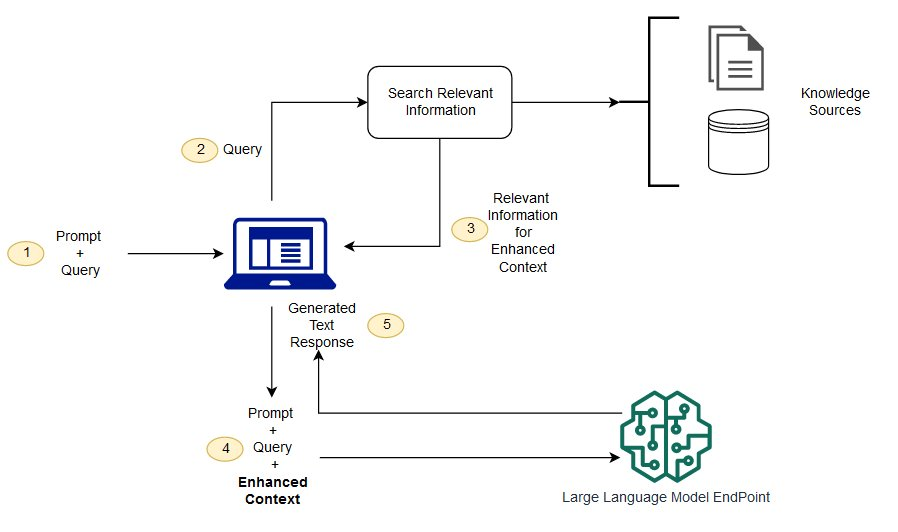
\includegraphics[width=\textwidth]{images/rag_workflow.jpg} 
  \caption{Retrieval-augmented generation pipeline combining user queries with external knowledge to produce context-aware responses.\\
  \footnotesize{Source: \url{https://aws.amazon.com/de/what-is/retrieval-augmented-generation/}.\nocite{noauthor_was_nodate}}}
  \label{fig:rag}
\end{figure}

\subsection{Pipeline Components and Common Practices}
The design of RAG pipelines can vary considerably depending on the specific use case, domain of application, and resources available. Still, a number of recurring practices have gradually crystallised into what can be regarded as the current state of the art in retrieval-augmented generation \citep{vaibhav_retrieval-augmented_2025,wang_searching_2024,arslan_survey_2024,gao_retrieval-augmented_2024,gupta_comprehensive_2024}. These practices often serve as reference blueprints rather than rigid prescriptions, since not every component needs to be implemented in every system. Instead, they represent a modular design space, where specific strategies can be combined, adapted or omitted to suit particular tasks.

In its most typical configuration, a RAG pipeline comprises the following tasks:
\begin{itemize}
  \item \textbf{Query understanding and classification.} Not all queries require retrieval from external sources. Advanced systems first analyse and classify incoming queries to determine whether retrieval is necessary or if the language model alone suffices. This step relies on natural language understanding (NLU) techniques to extract key entities, relationships, and user intent, thereby improving efficiency and reducing unnecessary retrieval latency.
    \item \textbf{Document indexing and chunking.} Raw data from source documents is preprocessed, cleaned, segmented into smaller chunks at token, sentence, or semantic level, and converted into dense vector representations called embeddings. Recent studies recommend dynamic or semantic chunking over simple fixed-size splitting, as it better preserves context and improves retrieval quality -- especially in heterogeneous domains \citep{gao_precise_2022}.
    \item \textbf{Embedding and Vector Database.} Both document chunks and user queries are embedded into a shared vector space using models fine-tuned for semantic similarity -- e.g., BAAI/bge, LLM-Embedder, intfloat/e5. These vectors are stored in vector databases -- e.g., Milvus, Faiss, Qdrant --,\footnote{Vector databases such as Milvus and Qdrant extend similarity search with native metadata management and distributed scalability. Milvus, built for large-scale applications, focuses on cloud-native deployment and support for multiple indexing strategies, making it suitable for enterprise environments \parencite{2021milvus,2022manu}. Qdrant, written in Rust, is designed for high-performance real-time search and offers particularly strong metadata filtering capabilities \citep{qdrant_github_nodate}. Faiss (Facebook AI Similarity Search)  is a high-performance library developed by Meta AI that focuses on efficient vector indexing and similarity search without built-in metadata handling \citep{douze2024faiss}. In research contexts, these characteristics can be advantageous: Faiss offers speed, flexibility, and a wide choice of indexing methods, while metadata can be managed externally (e.g., through a separate mapping file), allowing full control over the experimental pipeline.} selected based on scalability, indexing strategy, and support for specific search capabilities.
    \item \textbf{Retrieval and query transformation.} When a user submits a query, it is first encoded into a vector representation and used to retrieve the top-$k$ relevant chunks from the indexed KB via similarity search. To make it more robust, the pipeline can adopt a hybrid approach based on dense retrieval -- embedding-based methods such as DPR or Contriever -- combined with sparse retrieval -- lexical methods such as BM25. Retrieval can be further improved through query transformation strategies, including rewriting, decomposition, or the generation of hypothetical supporting documents -- e.g., HyDE.
    \item \textbf{Reranking.} the initial candidate set can be reordered to emphasise relevance to the original query. This is frequently achieved with cross-encoder models -- such as monoT5, monoBERT, or RankLLaMA --, which jointly consider the query and each candidate, or with more sophisticated algorithms through heuristics. This contextualization ensures that the most pertinent information is prioritised for the generative model.\\See \autoref{tab:rerank_algorithms} for a summary on reranking techniques.
    \item \textbf{Repacking and summarization.} In some cases, retrieved passages may be reorganised or summarised to distil key information, especially when dealing with lengthy corpora. This step can involve extractive summarization or abstractive -- e.g., with Pegasus -- techniques to condense information and fit within the context window of the generator model.
    \item \textbf{Generation.} The generative model -- usually a transformer-based LLM such as T5, BART, or GPT -- synthesises a response conditioned on both the original query and the retrieved context, integrating intrinsic model knowledge with external evidence to produce a coherent, accurate, and contextually grounded answer.
\end{itemize}


\autoref{tab:best_rag} presents an overview of the methods most consistently reported as high-performing for each module of a RAG pipeline. When aiming for balanced efficiency -- i.e., reducing latency while maintaining good, but not maximal, accuracy -- adjustments are typically made at the retrieval and reranking stages. In practice, this involves replacing the Hybrid + HyDE retrieval method with a standard Hybrid search approach, which combines BM25 and dense retrieval without pseudo-document generation, and substituting monoT5 with TILDEv2 for reranking, which delivers faster processing at the cost of a modest reduction in answer quality \citep{wang_searching_2024}.

\addtocounter{table}{-1}
\begin{table}[H]
\centering
\footnotesize
\begin{tabularx}{\textwidth}{l X}
\toprule
\textbf{Algorithm} & \textbf{Rationale} \\
\midrule
Cross-encoder rerankers & Jointly encode concatenated query-document pairs to produce fine-grained relevance scores. These models -- e.g., monoT5, monoBERT, RankLLaMA -- are fine-tuned to classify relevance as ``true'' or ``false'', and at inference, documents are ranked by the predicted probability of the ``true'' label \citep{wang_searching_2024}. \\
\cmidrule(lr){1-2}
TILDE \citep{zhuang_tilde_2021} & Token-level likelihoods for queries across a collection, allowing fast reranking by summing the probabilities of query tokens given each candidate passage. \\
\cmidrule(lr){1-2}
Learning-to-Rank (LTR) \citep{gupta_comprehensive_2024} & Traditional machine learning ranking approaches: \textbf{a) Point wise:} predicts relevance score for each document independently; \textbf{b) Pair wise:} compares pairs of documents to learn relative relevance; \textbf{c) List wise:} considers the entire ranked list at once.\\
\cmidrule(lr){1-2}
HyDe \citep{gao_precise_2022}  & Generates hypothetical documents from queries for dense retrieval.\\
\cmidrule(lr){1-2}
Hybrid Search (sparse + dense scoring) & Blends scores from dense retrievers (semantic similarity -- e.g., DPR, Contriever) and sparse methods (lexical overlap -- e.g., BM25, TF-IDF) for robust ranking. Sometimes uses learnable weighting \citep{wang_searching_2024}. \\
\cmidrule(lr){1-2}
HyDE + Hybrid Search \citep{wang_searching_2024} & Combines HyDE's hypothetical document generation with hybrid search for retrieval. \\
\cmidrule(lr){1-2}
Graph-based \citep{han_retrieval-augmented_2025} & Constructs a graph of candidates (nodes) based on relationships (semantic, citation, or knowledge graph edges), then uses graph algorithms  (e.g., PageRank, label propagation) to identify central passages. \\
\cmidrule(lr){1-2}
Self-RAG (LLM-enhanced reranking) \citep{asai_self-rag_2023} & Uses LLMs directly to score or select the most relevant passages, sometimes via few-shot prompting or chain-of-thought reasoning. \\
\bottomrule
\end{tabularx}
\vspace{0.5em}
\caption{Algorithms for document retrieval and reranking in RAG pipelines}.
\label{tab:rerank_algorithms}
\end{table}



\addtocounter{table}{-1}
\begin{table}[H]
\centering
\begin{tabularx}{\textwidth}{l>{\raggedright\arraybackslash}X>{\raggedright\arraybackslash}X}
\toprule
\textbf{Module}         & \textbf{Method(s)} & \textbf{Functionality} \\
\midrule
Retrieval         & Hybrid with HyDE            & Combines Hybrid Search (BM25 + dense) and HyDE pseudo-documents. \\
\cmidrule(lr){1-3}
Reranking         & DLM w/ monoT5                      & Deep LLM-based reranker (good balance of quality and speed). \\
\cmidrule(lr){1-3}
Chunking          & Small2big / Sliding Windows & Organising chunk block relationships for context preservation. \\
\cmidrule(lr){1-3}
Embedding         & LLM-Embedder                & Dense supervised retriever, best trade-off performance/size. \\
\cmidrule(lr){1-3}
Vector Database   & Milvus                      & Best coverage of index type, scalability, hybrid search, cloud-native. \\
\cmidrule(lr){1-3}
Repacking         & Reverse                     & Puts most relevant context close to the query. \\
\cmidrule(lr){1-3}
Summarization     & Recomp                      & Both extractive and abstractive methods tested; Recomp performs best. \\
\bottomrule
\end{tabularx}
\vspace{0.5em}
\caption{Best-performing RAG pipeline configurations across modules, selected for maximising performance w.r.t. answer quality and accuracy.}
\label{tab:best_rag}
\end{table}

\autoref{fig:summary_rag} provides a broader overview of the RAG ecosystem. The paradigm evolves from naive to modular RAG, incorporating techniques for improving retrieval and generation -- e.g., chunk optimization, adaptive retrieval, dual fine-tuning --, as well as the key issues of when, what, and how to retrieve. RAG also faces open challenges, including robustness, scaling laws, production readiness, alongside modality extensions to image, audio, video, code, and ecosystem directions like customization, specialization. Finally, current evaluation targets and frameworks distinguish between retrieval quality and generation quality, together with their assessment aspects such as answer relevance, context relevance, faithfulness, robustness, and integration \citep{gao_retrieval-augmented_2024}.

\begin{figure}[H]
  \centering
  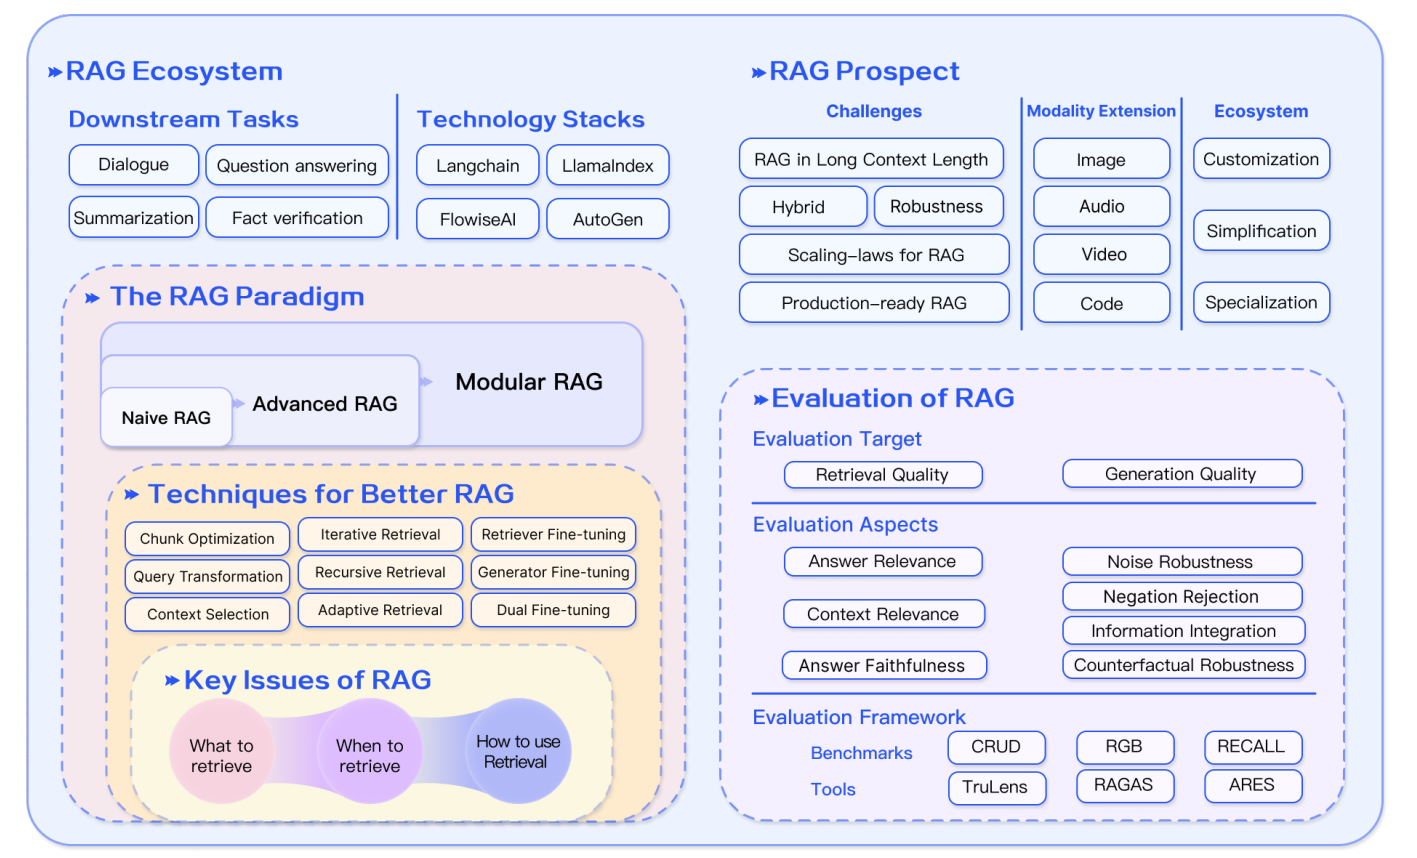
\includegraphics[width=\textwidth]{images/RAG_ecosystem.png} 
  \caption{Summary overview of the RAG ecosystem.\\
  \footnotesize{Source: \cite{gao_retrieval-augmented_2024}}.}
  \label{fig:summary_rag}
\end{figure}

\subsection{Evaluation and Benchmarking}\label{sec:eval_and_bench}
Evaluating RAG systems poses unique challenges, as traditional metrics like BLEU, ROUGE or METEOR may not fully capture the quality of generated responses, particularly in terms of factual accuracy and contextual relevance \citep{deriu_survey_2020}. In conversational QA research, this limitation has long been acknowledged, as multi-turn settings require models to answer a single query and to maintain consistency, resolve co-references, and adapt to evolving conversational context \citep{zaib_conversational_2022}. Consequently, evaluation must go beyond surface level overlap and incorporate measures that reflect contextual appropriateness and understanding at discourse level. Moreover, assessing RAG systems requires attention to both retrieval and generation quality, since failures in either stage directly impact the final response \citep{abeysinghe_challenges_2024}.

Surveys of the field increasingly stress the need for frameworks capable of measuring multiple dimensions of RAG. Despite the rapid advancements in retrieval, generation, and augmentation, evaluation methods remain underdeveloped, with persistent challenges in capturing retrieval quality, hallucination rates, and faithfulness of generated content in a systematic way \citep{gao_retrieval-augmented_2024}. Large-scale benchmarks such as TREC \citep{voorhees_trec_2005}, MS MARCO \citep{bajaj_ms_2018} and BEIR \citep{thakur_beir_2021} continue to be standard for retrieval, but generation quality requires different approaches. Newer frameworks like the \textit{Retrieval-Augmented Generation Assessment System (RAGAS)} have therefore been introduced to capture aspects such as contextual alignment, answer faithfulness, and pipeline-level performance \citep{es_ragas_2023}.

Experimental studies of RAG pipelines within LLM-based applications further demonstrate the complexity of the task. For example, a recent work compares automated metrics, human evaluation, and LLM-based evaluation in the context of \textit{EdTalk}, a RAG-powered chatbot built to navigate educational reports. Their findings show that automated metrics such as BLEURT are useful for rapid iteration but often misalign with human judgments, while factored human evaluation -- structured around criteria including correctness, informativeness, relevance, clarity, and hallucination -- provides richer insights into system performance. At the same time, LLM-based evaluators show promise for scalable assessment but risk inflating scores, especially when the same model is used for both generation and evaluation. This stresses the need for hybrid and carefully designed evaluation pipelines when deploying RAG in real-world contexts \citep{abeysinghe_challenges_2024}.

Human-in-the-loop assessment remains indispensable, with expert judges assessing criteria such as factual accuracy, coherence, and domain relevance -- offering richer and often more reliable quality assessments than quantitative metrics alone. In conversational contexts, this is especially important, as metrics must reflect user satisfaction and interaction quality rather than isolated response correctness \citep{gupta_comprehensive_2024}.

Alongside automated and human-centred metrics, evaluation taxonomies are moving toward a more fine-grained view of system quality. Dimensions such as answer relevance, context relevance, and faithfulness directly address hallucination and grounding, while robustness dimensions -- including resilience to noise, negation, counterfactual scenarios, and multi-source information integration -- test whether systems remain reliable under real-world conditions. To operationalise these dimensions, new benchmarks such as CRUD, RGB, and RECALL extend beyond traditional IR settings by jointly assessing retrieval and generation. Complementary tools make evaluation continuous and developer-friendly: RAGAS targets faithfulness and contextual alignment, ARES offers flexible automated pipelines, and TruLens integrates performance monitoring into deployed workflows \citep{gao_retrieval-augmented_2024}.

Furthermore, ethical considerations must be embedded throughout the lifecycle of RAG pipelines. Protecting data privacy, mitigating algorithmic bias, and complying with regulations such as GDPR are fundamental. This means adopting technical measures like privacy by design, data minimisation, and access control, in addition to committing to broader ethical principles widely recognised in international guidelines: transparency, justice and fairness, non-maleficence and responsibility \citep{jobin_global_2019}. Ongoing audits, stakeholder involvement, and mechanisms for accountability, including whistleblowing and legal clarity, help bridge the gap between abstract principles and operational practice, ensuring systems remain trustworthy and socially beneficial \citep{ashery_emergent_2025}.

Overall, the line of evolution of RAG systems points toward increasingly sophisticated applications that are deeply integrated into the workflows of research, industry, and cultural institutions. Innovations in evaluation frameworks, user interaction, and system scalability are steadily pushing the boundaries of what these models can achieve. As these technologies continue to mature, success will depend on the ability to combine robust benchmarking, user-centred feedback mechanisms, and adaptive optimisation strategies. Overcoming challenges related to factuality, scalability, and responsible deployment will be essential for building trustworthy systems capable of delivering high-quality information in context-sensitive settings. Looking ahead, continued advances in RAG are set to play a pivotal role in shaping the future of digital knowledge access and discovery, and establish it as a cornerstone technology \citep{zaib_conversational_2022,wang_searching_2024, gao_retrieval-augmented_2024}.

\section{New Frontiers Applications}\label{sec:evol_qas}
RAG systems are increasingly deployed across a wide spectrum of contexts -- spanning academic research, enterprise infrastructures, and real-world product environments -- where they serve to enhance data accessibility, support decision-making, and facilitate natural language interaction with complex KBs. Recent surveys and empirical studies trace a rapidly expanding set of scholarly applications. In the context of academic support, for instance, retrieval-augmented pipelines power automated literature review tools and citation management platforms such as \textit{LitLLM} \citep{agarwal_litllm_2025}, and \textit{KNIMEZoBot} \citep{alshammari_knimezobot_2023}. In conversational AI, advanced retrieval enables grounded multi-turn dialogue, exemplified by \textit{Wizard of Wikipedia (WoW)} \citep{dinan_wizard_2019}, which can be read as an early instantiation of what is now formalised as RAG-based dialogue modelling. The paradigm is also leveraged for large-scale summarisation, distilling insights across vast corpora of scholarly papers, and for fact verification tasks, as in resources like \textit{PubHealth}, increasingly adopted to counter misinformation in sensitive domains such as health communication \citep{kotonya_explainable_2020}. In this regard, RAG has proven especially valuable in domain-specific knowledge extraction, most notably in biomedical and legal research, where retrieval mechanisms act as an extension of expert knowledge.


In one experiment, a RAG system was developed to assist data scientists through a combination of GROBID library\footnote{GROBID is a machine learning library designed to extract, parse, and convert raw documents, like PDFs, structured XML/TEI encoded documents \citep{GROBID}.} for structured bibliographic extraction, fine-tuned embeddings, semantic chunking, and an abstract-first retrieval strategy. The system's performance, assessed using RAGAS, demonstrated improved faithfulness and context relevance in response generation \citep{aytar_retrieval-augmented_2024}. A similar approach was explored in the context of academic library systems, where RAG was applied to improve contextual retrieval through semantic indexing of structured metadata -- e.g., MARC/RDA standards -- and multimodal resources. Additionally, the framework introduced conversational querying via a natural language interface, supporting compound interdisciplinary searches and significantly improving document discoverability by synthesising citation-backed responses from diverse scholarly sources -- including journals, datasets, and videos; this solution also addressed challenges such as copyright compliance and ethical AI transparency \citep{bevara_prospects_2025}.  Collectively, these studies affirm the efficacy of RAG systems in alleviating information overload and improving research workflow discoverability.

In parallel, further critical insights into the design of RAG systems for domain-specific and technical content have been highlighted in recent work \citep{soman_observations_2024}, which closely aligns with the methodological framework adopted in the GNA question-answering system. Using IEEE telecommunications engineering corpora -- i.e., wireless LAN specifications and battery glossaries -- as testbeds, their analysis highlights key factors influencing retrieval quality, which include chunk size, sentence-level similarity, and the strategic placement of domain-specific terms. These aspects are similarly addressed in the GNA RAG pipeline \citep{pograri_question-answering_2025}, which applies customised chunking, semantic preprocessing, and contextual embedding strategies. Both studies advocate for more nuanced and contextually informed approaches to enhance precision in technical and highly structured domains.

Numerous recent graduate-level research projects have provided substantive input into the implementation and evaluation of RAG systems:
\begin{itemize}
    \item \textcite{antolini_experimental_2025} developed a custom RAG system for open-domain question answering using both traditional (BM25, PRF) and advanced retrieval strategies, integrated with local LLMs. A novel Parametric RAG (PRAG) approach was also explored, embedding context into model parameters for performance gains;
    \item \textcite{caramanna_progettazione_2024} investigated conversational agent architectures, comparing various LLM types and retrieval configurations;
    \item \textcite{florio_progettazione_2024} implemented a LangChain-based RAG chatbot for corporate documentation, evaluating multiple vector database technologies.
    \item \textcite{salcuni_utilizzo_2025} applied RAG to the medical domain, improving LLM responses in hypertension care. The study used RAGAS to assess quality and relevance, focusing on personalization and accuracy;
    \item \textcite{nicoletti_llms_2025} developed Essence Coach, a chatbot that integrates LLMs with the Essence software engineering standard. This system significantly outperformed generic LLMs like GPT-4o in domain-specific reasoning tasks.
\end{itemize}

\section{Retrieval-Augmented Generation in the Digital Humanities}\label{sec:rag_dh}
A growing body of research is exploring RAG applications within the digital humanities. One such example is the \textit{iREAL} project, which applied RAG to interpret archival records from Aboriginal schools in Australia, demonstrating a careful balance between cultural sensitivity and historical accuracy \citep{callaghan_prototyping_2025}. Another initiative, \textit{ValuesRAG}, focuses on cultural alignment in LLMs by integrating societal and demographic knowledge through retrieval-augmented contextual learning, experimenting with the \textit{World Values Survey} dataset \citep{seo_valuesrag_2025}. In another case, the \textit{Foggia Occupator Dataset} project applied a RAG model to post-WWII Italian periodicals, extracting information on political figures and stylistic traits \citep{ciletti_retrieval-augmented_2025}.

Among the technical approaches explored in recent experiments on generative AI for digital scholarly editions (DSEs), RAG emerges as a promising method for addressing challenges such as entity linking (EL) and the integration of external knowledge sources. Notably, RAG is recognised for its ability to mitigate hallucinations in named entity recognition (NER) and to enable the enrichment of text with information from structured databases or knowledge graphs \citep{pollin_when_2025}. For example, an experiment with the \href{https://www.regesta-imperii.de/en/home.html}{Regesta Imperii project}\nocite{noauthor_home_nodate} demonstrates how knowledge bases, including Neo4j graph databases, are leveraged within RAG pipelines to improve accuracy in information extraction, entity normalization, and semantic annotation \citep{kuczera_chatgpt_2024}. Similarly, the editorial workflow developed for the \href{https://web.archive.org/web/20241120122545/https://gams.uni-graz.at/context:hsa}{Hugo Schuchardt Archive} outlines a process that combines prompt engineering, human-in-the-loop oversight, and RAG tool chains to enhance the generation of TEI-compliant XML, supporting more explainable and modular processing pipelines \citep{pollin_new_2023}. These and other experiments underscore the need for standardised workflows, robust evaluation protocols, and systematic research into both the strengths and weaknesses of LLMs and related tools in the editorial process, while also advocating for thoughtful engagement with advanced computational methods in the humanities \citep{pollin_workshop_2024}. As digital editions become increasingly complex and interconnected with broader knowledge infrastructures, the relevance and application of AI technologies such as RAG are both expected and desirable to grow accordingly.

RAG methodologies are being adopted within the GLAM sector as well. In archival contexts, a smart assistant developed for querying the \textit{Prozhito} digital archive of personal diaries combines text-to-SQL filtering, hybrid search, and automatic query reformulation, proving especially effective for historians and anthropologists without prior knowledge of database query languages  \citep{sergeev_talking_2025}. Meanwhile, in museum settings, a comparative evaluation of RAG techniques versus direct large-context input approaches -- i.e., feeding the entire context at once to a language model -- for answering multimodal questions about artworks demonstrated that large-context models generally give more accurate answers than RAG, at least for this task and dataset. However, RAG remains useful when information exceeds context window limits or when efficiency is important \citep{ramos-varela_context_2025}.

Innovations in graph-based retrieval are also gaining momentum. Techniques combining structured supervision and chain-of-thought prompting have been used to map character relationships in early modern English historiography, thereby reducing the manual workload typically associated with historical data annotation \citep{fan_research_2025}. Related directions are being explored within cultural heritage institutions, as seen in the \textit{CAT-IA} initiative, which integrates ArCo knowledge graph \citep{carriero_arco_2019} within a RAG system for provenance tracking, AI explainability (XAI), and structured metadata extraction \citep{barbato_nasce_2025}. Designed to streamline and enrich user interactions with the General Catalogue of Cultural Heritage \textit{(Catalogo generale dei beni culturali)}, \textit{CAT-IA} marks a notable stride in applying advanced digital technologies to promote accessibility and valorization of cultural assets.

A complementary, conceptual perspective emerges in a critical mapping of the theoretical contours of RAG within the broader landscape of archives, libraries, and cultural heritage, articulating the potential for RAG-augmented LLMs to enhance the precision, accessibility, and contextualization of information retrieval, and foregrounding the social and infrastructural challenges inherent in such integration. This viewpoint encourages the field to reflect on both the affordances and the epistemic and ethical complexities introduced by RAG systems in digital humanities contexts \citep{di_marcantonio_intelligenza_2024}.


Finally, efforts to advance access to fragmented digital repositories -- such as web archives -- have increasingly adopted RAG methodologies. An illustrative bespoke prototype transforms keyword-based search into semantically guided question answering \citep{davis_unlocking_2025}, sharing architectural parallels with the GNA QA system presented in the context of this thesis. Both systems prioritise semantic retrieval over lexical matching using dense embeddings -- e.g., \textit{E5} variants \citep{wang_text_2024} -- to interpret queries in context, employ structured text processing pipelines to reduce noise in source materials, and apply optimised chunking strategies for retrieval accuracy. Crucially, these studies highlight RAG’s potential to transform scattered and heterogeneous resources -- whether web archives or catalographic procedures -- into coherent, accessible knowledge through contextual synthesis.

\section{Future Directions}
Ongoing research is rapidly pushing the frontiers of RAG, opening up new avenues  that extend well beyond traditional information retrieval into domains such as scientific research and the digital humanities. Among the most promising innovations, is the use of synthetic corpora to bolster the robustness and generalizability of RAG systems, particularly in low-resource or specialised domains where annotated data is scarce \citep{bor-woei_generative_2024}. This strategy improves retrieval accuracy while addressing longstanding issues of bias, coverage, and representativity in humanities corpora. 

RAG is also at the core of a new wave of applications that automate and enhance scholarly practices. In scientific research, advanced RAG frameworks -- including agentic systems like \textit{PaperQA} \citep{lala_paperqa_2023} -- are being leveraged to conduct systematic literature reviews, automate evidence synthesis, summarise emerging trends, and provide transparent citation recommendations. Particularly, these multi-stage architectures enable recursive reasoning and dynamic tool usage, often surpassing human-level performance in both retrieval and summary tasks \citep{skarlinski_language_2024}. 

Despite these advances, several critical research challenges remain. There is an urgent need to develop domain-adapted and multilingual LLMs that can process not just text, but also multimodal data such as images, tables, and audiovisual materials -- a key requirement for both scientific and cultural heritage applications. Future RAG systems should be able to retrieve and reason over heterogeneous, cross-domain sources, necessitating robust mechanisms for evaluation, source citation, multimodal fusion, and trust calibration. The ongoing development of benchmarks and evaluation datasets, tailored to the peculiar needs of fields such as the digital humanities, is essential to guide progress and ensure methodological rigour \citep{yue_survey_2025}.

Another major direction is the semantic enrichment of RAG pipelines through the integration of ontologies and knowledge graphs. Ontologies, as formal domain knowledge models, provide structured frameworks that enable more precise and explainable retrieval semantic coherence, and the inclusion of ethical dimensions in generative AI. Complementing this, knowledge graphs capture complex relationships and support context-aware multi-hop reasoning, improving accuracy, explainability, and cultural sensitivity of outputs. Current research and practical applications in this direction span a range of initiatives, from ontology-guided entity typing to the grounding of AI in explicit ethical and procedural knowledge, demonstrating that these semantic tools are essential for creating robust and transparent RAG systems, addressing challenges in fields as diverse as healthcare, engineering, scientific discovery, and enterprise knowledge management \citep{tiwari_ontorag_2025, ludwig_ontology-based_2025, bran_ontology-retrieval_2024, sharma_og-rag_2024, xiao_orag_2024, park_ontology-based_2024, debellis_integrating_2024,franco_ontology-based_2020}.

In the specific context of the digital humanities, the accelerated adoption of AI is shaping a transformative future for scholarship, curation, and access to cultural heritage. The diverse case studies and technical innovations, discussed in \autoref{sec:rag_dh}, illustrate both the breadth of RAG’s impact and the field’s growing ambition. Across applications, from DSEs, to archival assistance and museum information systems, RAG is emerging as a pivotal enabler for addressing the limitations of traditional search and annotation by supporting contextually grounded, semantically rich, and explainable information access.

Looking forward, several converging trends and open challenges will define the evolution of RAG in the digital humanities. First, technical advances such as the integration of knowledge graphs, graph-based retrieval, and multimodal pipelines are driving improvements in semantic linking and annotation of historical, literary, and artistic materials. Second, the increasing complexity of digital scholarly editions and GLAM infrastructures is catalysing demand for standardised, reproducible workflows, robust evaluation protocols, and domain-adapted benchmarks, ensuring that RAG methods are critically assessed and tuned for the nuanced needs of humanistic research.

At the same time, as digital repositories become ever more fragmented, the promise of RAG lies in its ability to synthesise heterogeneous, dispersed data, transforming scattered web archives, periodicals, and catalogues into knowledge spaces that are accessible and meaningfully structured. Yet, this evolution also foregrounds critical conceptual and ethical questions. As highlighted by recent critical perspectives, it is essential to position RAG as an augmentative technology: one that enhances, but does not replace, established cataloguing, metadata, and interpretive practices. Human interpretive oversight, transparency, and cultural sensitivity must remain central, particularly as RAG systems are increasingly relied upon for knowledge production and mediation in complex social and historical domains \citep{di_marcantonio_intelligenza_2024}.

In sum, the next phase of RAG’s development in the digital humanities will require sustained interdisciplinary collaboration and critical reflection. Researchers and practitioners must continue to experiment with new strategies, but also engage deeply with the epistemic, social, and infrastructural complexities of integrating advanced AI into cultural knowledge management and disciplines. Ultimately, RAG applications stand poised not only to offer improved access to information, but they also invite a reimagining of the relationship between artificial intelligence and cultural knowledge production, fostering tools that augment -- not displace -- human creativity and understanding.
\end{spacing}
\chapter{Case Study: A Question-Answering System for GNA}
\label{chap:casestudy}
\sloppy
\begin{spacing}{1.5} 

\section{Geoportale Nazionale per l’Archeologia (GNA)}
Geoportale Nazionale per l'Archeologia (GNA) \citep{mic_mic_2019} serves as the central online hub for the collection, management, and dissemination of data generated by archaeological investigations carried out across Italy \citep{acconcia_pubblicazione_2023}. Developed under the auspices of the Ministry of Culture (MiC), the project's primary goal is the creation of a dynamic archaeological map of the national territory, which is easily updatable over time, openly accessible, and designed for reuse and integration across multiple institutional and disciplinary contexts \citep{falcone_dematerializzazione_2023}.

The inception of the GNA traces back to a 2014 \textit{Memorandum of Understanding} signed by the Ministero dei Beni e delle Attività Culturali e del Turismo (MiBACT) -- specifically the Segretariato Generale, the Direzione Generale per le Antichità (DG-Ant), and the Consiglio Nazionale delle Ricerche (CNR). This agreement laid the groundwork for a national platform dedicated to the safeguarding and enhancement of cultural heritage through integrated digital infrastructure. However, it was the establishment of the Istituto Centrale per l’Archeologia (ICA) in 2016 that provided the structural and institutional foundation for the GNA. The ICA’s mandate to define standards and promote digital archaeological databases gave renewed potential to the initiative, which culminated in the launch and formal presentation of the GNA at a ministerial venue in 2019 \citep{calandra_il_2023}.

Beyond being a data aggregator, the GNA serves as a dynamic knowledge base, collecting digital content from professional archaeologists -- especially those engaged in preventive archaeology --, research groups, universities, and concession-holders. The platform also accommodates a variety of outputs, from QGIS-based vector data to reports, documentation packages, and datasets from academic and research contexts. Data publication in the GNA is managed with attention to quality standards, intellectual property, and open-access principles, supported by the assignment of DOIs and the use of Creative Commons licensing (CC-BY 4.0), ensuring both traceability and reusability \citep{acconcia_pubblicazione_2023,falcone_dematerializzazione_2023,boi_il_2023}.

\subsection{Purpose and Scope}
As the official repository for all research activities in archaeology -- particularly those related to public infrastructure projects -- the GNA platform was established to provide a unified national access point to essential archaeological data gathered nationwide. This includes the interventions listed in \autoref{tab:gna_data_sources}, all conducted under the scientific supervision of the Italian Ministry of Culture (MiC) \citep{acconcia_pubblicazione_2023,falcone_dematerializzazione_2023}.

\addtocounter{table}{-1}
\begin{table}[H]
\centering
\footnotesize
\begin{tabularx}{\textwidth}{ l >{\justifying\noindent\arraybackslash}p{0.65\textwidth} }
\toprule
\textbf{Archaeological interventions} & \textbf{Description} \\
\midrule
Preventive archaeology reports & Data from excavations and surveys carried out ahead of construction projects (e.g., highways, railways, pipelines), often submitted by private firms or cultural heritage consultants. \\
\cmidrule(lr){1-2}
Assisted scientific excavations records & Results from academic digs by universities or research institutions, including documentation of stratigraphy, finds, and site interpretation. \\
\cmidrule(lr){1-2}
Accidental discoveries & Locations of fortuitous archaeological finds, such as during agricultural work or construction, reported to local heritage authorities. Typically include preliminary spatial data and descriptive reports. \\
\cmidrule(lr){1-2}
Scheduled excavations & Long-term planned investigations, often at known heritage sites, including geospatial boundaries, uncovered structures, and findings. \\
\cmidrule(lr){1-2}
Archaeological surveys & Surface survey data with GPS-tracked locations of finds, artifact scatters, and site features. \\
\cmidrule(lr){1-2}
Cultural heritage GIS layers & External datasets from institutions (regional superintendencies, local governments, ICCD), e.g., maps of protected zones, risk maps, or site inventories. \\
\cmidrule(lr){1-2}
Legacy data and digitised archives & Georeferenced digitizations of paper maps, notebooks, and archival records previously stored in non-digital formats, essential for integrating historical with current data. \\
\cmidrule(lr){1-2}
Depository locations & Georeferenced storage locations of archaeological finds (museums, storerooms) associated with sites or interventions. \\
\cmidrule(lr){1-2}
Remote sensing and aerial surveys & Drone imagery, LiDAR scans, or satellite data used to identify and map archaeological features not visible at ground level. \\
\cmidrule(lr){1-2}
Paleontological sites & A specific level dedicated to paleontological sites is currently under study for future inclusion, aiming to protect this fragile heritage. \\
\bottomrule
\end{tabularx}
\vspace{0.5em}
\caption{Types of archaeological data sources integrated into Geoportale Nazionale per l'Archeologia.}
\label{tab:gna_data_sources}
\end{table}

\noindent These sources, once georeferenced and structured, are integrated into the GNA using standardised metadata and visualization protocols, to allow users to view, search, and analyse information in a spatially accurate and coherent manner \citep{boi_il_2023, acconcia_pubblicazione_2023}.

\subsection{Stakeholders and Intended Users}\label{sec:gna_plugin}
The development of the GNA saw significant acceleration during the COVID-19 pandemic, which provided both the urgency and institutional impetus toward the creation of a unified digital platform for managing archaeological data nationwide. This initiative built upon years of prior collaboration between key stakeholders, including the Istituto Centrale per l’Archeologia (ICA) and the Istituto Centrale per il Catalogo e la Documentazione (ICCD), who had already developed a cataloging structure to document archaeological assessments and identified sites within the Sistema Informativo Generale del Catalogo (SiGECweb) \citep{calandra_il_2023, boi_il_2023}. The pandemic underscored the limitations of purely textual cataloguing and catalysed a shift toward a more dynamic and geospatially grounded approach, leading to the adoption of a GIS-based framework better suited for preventive archaeology and territorial planning. The result was a consolidated national infrastructure designed not only to support compliance with cultural heritage protection regulations but also to enable data harmonization across previously fragmented practices \citep{acconcia_pubblicazione_2023}.

The GNA is primarily intended for use by:
\begin{itemize}
    \item Public administrators and government officials;
    \item Professional archaeologists and cultural heritage consultants;
    \item Stakeholders involved in public works, such as national infrastructure planners.
\end{itemize}

\noindent For instance, major entities like TERNA (the national electricity grid operator), RFI (the Italian railway network), or the Milan Metro rely on the platform to assess archaeological constraints before launching construction projects. The platform helps them identify archaeological sites, deposits, and or protected areas that must be preserved. The GNA also supports compliance with European and Italian open data and transparency regulations, guaranteeing both civic access and the protection of intellectual property, as per national FOIA and EU directives\footnote{The FOIA (Freedom of Information Act) Guidelines are documents issued by the Italian National Anti-Corruption Authority (ANAC) to clarify and guide the implementation of the right to generalised civic access in Italy. The guidelines -- especially those from 2016 -- define the limits and exclusions to access, as well as specify the publication and transparency obligations for public administrations.\\Read more at \url{https://foia.gov.it/normativa}.\nocite{noauthor_normativa_2016}} \citep{falcone_dematerializzazione_2023}.

Central to the system is a QGIS\footnote{QGIS is a free, open-source Geographic Information System (GIS) software used for creating, managing, and analysing geospatial data.} template that standardises data entry and visualization. This tool supports collaborative integration of local information into the national infrastructure, offering users a unified territorial overview. It enables the comparison of diverse archaeological records, improves the quality of evaluations, and promotes transparency across institutional workflows. Thanks to its open-source foundation and modular structure, the GNA continues to evolve based on user feedback, maintaining a shared national standard while accommodating diverse local contributions \citep{calandra_il_2023, boi_il_2023}.

\subsection{User Manual and Operational Support}
To guide users in correctly navigating the system, a collaboratively maintained user manual (\textit{manuale operativo}) is made available online through a MediaWiki environment hosted on the GNA server \citep{gna_wiki_2024}. This living document offers structured instructions on all aspects of data input, visualization, and management within the GNA platform.

The manual offers step-by-step instructions for compiling and submitting data using the QGIS template, including the creation and editing of project modules (MOPR), the documentation of archaeological sites and events (MOSI), and the proper use of supporting layers such as risk maps or thematic overlays. Each section of the manual is designed to be accessible both to GIS beginners and to experienced professionals, offering annotated screenshots, workflow examples, and direct links to downloadable resources. A notable feature of the operational manual is its integration with the GNA QGIS plugin, which allows users to directly download standardised data layers -- such as archaeological risk assessments, site boundaries, or previous project records -- into their local GIS environment \citep{gabucci_template_2023}.

In addition to the written documentation, the GNA provides ongoing operational support through a dedicated Help Desk service, coordinated by Ada Gabucci.\footnote{Ada Gabucci is a specialist in Roman-period archaeology, with expertise in stratigraphic methods, northern Italian material culture, and the structuring of archaeological data. She has over thirty years of experience consulting for public institutions, including the Italian Ministry of Culture (ICCD, ICA, DG-ABAP), its regional branches, the Veneto Region, and several universities, including Trieste, Venice, Verona, Bologna, Genova, and Pisa. Her work also encompasses cultural heritage cataloguing, ministerial regulations, and the design of complex Geographic Information Systems.\\Source: \url{https://web.archive.org/web/20250724081422/https://conf24.garr.it/it/speaker/ada-gabucci}.\nocite{noauthor_ada_2025}} Users encountering technical challenges or seeking clarification on data entry procedures can contact the Help Desk for personalised assistance. This direct support, together with the collaborative and evolving nature of the manual, fosters a strong community of practice, encouraging the sharing of expertise and continual improvement of the platform’s tools and resources.

\section{Proof of Concept}
In response to the challenges users face in quickly locating relevant information when accessing and navigating the GNA operative manual, as well as the high volume of inquiries received by the Help Desk, a need emerged for a smarter and more efficient support solution. To address this, we developed an information system in the form of a question-answering system designed to assist users directly and reduce the Help Desk’s workload. Based on the current state of AI, ML and DH methodologies -- as discussed in \autoref{chap:sota} and especially \autoref{sec:evol_qas} -- RAG combined with NLP was chosen as the most effective approach. This technology enables the chatbot to dynamically retrieve relevant information, which serves as an augmented knowledge base, allowing it to generate precise, context-aware, and up-to-date answers tailored to user queries.

\subsection{Functional Requirements}
Functional requirements define what the system must do to deliver value to users and stakeholders:
\begin{itemize}
    \item \textbf{Natural language understanding (NLU):} the system must interpret user queries phrased in natural language, supporting diverse question types (factoid, list, explanatory, etc.) and handling both simple and complex multipart queries.
    \item \textbf{Information retrieval:} the system must retrieve relevant passages or document segments from the GNA knowledge base, using vector similarity search over chunked content.
    \item \textbf{Context-aware answer generation:} the system must synthesise coherent, context-aware answers using RAG, drawing from retrieved passages and maintaining reference to original sources.
    \item \textbf{Source attribution and citation:} answers must include traceable citations (e.g., URLs) to ensure transparency and support verification.
    \item \textbf{Conversational memory:} the system must retain context from previous exchanges to handle follow-up questions and maintain dialogue continuity within a session.
    \item \textbf{Multilingual support:} the chatbot must process and generate responses in Italian, with potential extensibility to other languages.
    \item \textbf{User feedback collection:} the system must provide mechanisms for users to rate responses and submit qualitative feedback, enabling ongoing evaluation and improvement.
    \item \textbf{Interactive user interface:} users must be able to input queries and view answers through an accessible web interface, including features such as clickable citations, feedback buttons, and session management.
\end{itemize}

\subsection{Non-Functional Requirements}
Non-functional requirements define how the system should operate to ensure quality, usability, and maintainability:
\begin{itemize}
    \item \textbf{Accuracy and relevance:} answers must be factually correct, directly address user queries, and reference up-to-date information.
    \item \textbf{Performance and scalability:} the system must deliver responses with low latency (target average retrieval and response time inferior to 1 second per query) and scale to support multiple concurrent users.
    \item \textbf{Robustness and reliability:} the system should gracefully handle invalid queries, errors, and resource constraints without crashing.
    \item \textbf{Transparency and traceability:} every generated answer must cite its sources clearly. The underlying process for retrieval should be auditable.
    \item \textbf{Security and privacy:} the system must securely handle sensitive data. User interactions should be anonymised, and no personally identifiable information should be stored.
    \item \textbf{Maintainability and extensibility:} The architecture must support modular updates (e.g., changing retrieval strategies), and facilitate maintenance, debugging, and future enhancements.
    \item \textbf{Resource efficiency:} the solution must operate efficiently within the limits of available hardware, minimising memory and compute consumption, especially for cloud deployment scenarios without GPU access.
    \item \textbf{User accessibility:} the web interface must be usable by non-technical users and meet accessibility standards (e.g., clear labelling, visual feedback, keyboard navigation).
    \item \textbf{Continuous evaluation:} the system must support automated and human-in-the-loop evaluation methodologies, generating reports on retrieval accuracy, answer quality, and user satisfaction over time.
\end{itemize}

\citep{abu_shawar_chatbots_2007,arslan_survey_2024,gupta_comprehensive_2024}\\


The following chapter details the methodological framework and practical steps undertaken during the development of the system, providing in-depth explanation of the design choices, technical architecture, data preparation, implementation and evaluation processes.


\end{spacing}
\chapter{Methodology}
\label{chap:methodology}
\pdfcomment{WIP}
\begin{spacing}{1.5}

\section{Prototype}
\pdfcomment{use of langchain, cf. Akkiraju et al. 2024}

\section{Full-scale implementation}

\section{Knowledge-Base Construction and Preprocessing}
\subsection{Sitemap Generation}
      - URL Discovery and Filtering
      - Crawling Policies and Content Parsing
\subsection{Document Crawling and Chunking}
      - Content Extraction and Semantic Preservation
      - Chunking Strategy and Metadata Enrichment
      - Special Content Handling (text/tables/images)
\subsection{Vector Embeddings and Storage}
      - Multilingual Embedding Model (multilingual-e5-large)
      - FAISS Index Optimization for Retrieval

\section{Candidates Retrieval}
\pdfcomment{
      APPROFONDIMENTO:\\
(wang_searching_2024) --> more on retrieval techniques experiments (e.g., hyde, graph, re-rank w/ cross-encoders, etc.), rivedi 
{hakdagli_hybrid_2024} --> hybrid retrieval
{mulani 2024 re-ranking}
}
      - Top-k Similarity Search
      - Document Grouping by Provenance

\section{Generation}
- open source and proprietary LLMs \citep{noauthor_open_2025}
      - Mistral NeMo LLM Configuration
      - Response Generation and Validation

      \subsection{Prompt Engineering Techniques}
      - System Instructions and Constraints
      - Dynamic Citation Handling

\section{User Interface}
- Streamlit Application
      - Session State Management
      - Asynchronous Query Processing
-Interaction Features
      - Inline Feedback Mechanism

\section{Feedback Management}
- Feedback Data Collection
- streamlit local collection

      - SQLite Database
      - Feedback Rating System (3-point Likert)
      - Automated GitHub sync
      - Conflict Resolution Protocols

\section{Resource Optimization Strategies}
\subsection{Memory Management}
      - Garbage Collection Routines
      - Caching Mechanisms
\subsection{Computational Constraints Mitigation}
      - CPU-Only Deployment Adaptations
      - Error Handling and Recovery

\section{Evaluation}

\pdfcomment{ Akkiraju (2024) fifteen RAG pipeline control points, empirical results on accuracy-latency tradeoffs between large and small LLMs. }


\end{spacing}
\chapter{Results}
\label{chap:results}
\begin{spacing}{1.5}

This chapter presents the results with regard to the evaluation of the RAG QA system across its two stages of development: the prototype and the full-scale implementation. 

Each followed a distinct evaluation protocol. For the prototype, responses were assessed through a dual strategy combining human annotation on a 5-point Likert scale -- measuring consistency, fluency, completeness, and relevance -- with automatic scoring from an external LLM (GPT-3.5), prompted as an evaluator. By contrast, the re-engineered system was tested on a synthetic collection of 508 single-hop and 908 combined queries automatically generated from the GNA operative manual. The assessment included intrinsic IR metrics -- Recall@, MRR, nDCG@, AP@, Latency --  to quantify retrieval performance, alongside qualitative human feedback, to capture user-facing quality. Feedback was collected systematically through in-interface ratings tasks: each response was labelled on a 3-point Likert scale -- 1-star equals ``poor'', 2-stars equals ``fair'', 3-stars equals ``good'' --, offering direct insight into the perceived relevance, completeness, and fluency of the generated answers.


\section{Prototyping Phase}
The prototype offered an initial proof of concept, validating that a RAG architecture could be applied to the GNA corpus. Although limited in scale, it provided important insights into feasibility.

The evaluation outcomes (\autoref{fig:proto_results}) show a clear profile: consistency was rated at the highest level ($\approx$ 5), indicating that generated answers rarely contradicted themselves. Relevance ($\approx$ 4.7) and fluency ($\approx$ 4.9) also scored strongly, confirming the system’s ability to generate both accurate and linguistically natural responses. Completeness, however, achieved slightly lower values ($\approx$ 4.6), pointing to occasional gaps in coverage where answers did not fully integrate all available evidence.

Performance testing further revealed practical constraints. Embedding generation averaged 31.2 seconds per batch, while query responses were returned in $\approx$ 1.26 seconds on average. Although response time was acceptable for interactive use, overall efficiency lagged behind production-ready deployments, especially under heavy load. 

In sum, the prototype confirmed the viability of a RAG-based QA approach, but also highlighted the need for more scalable retrieval infrastructure.

\begin{figure}[H]
  \centering
  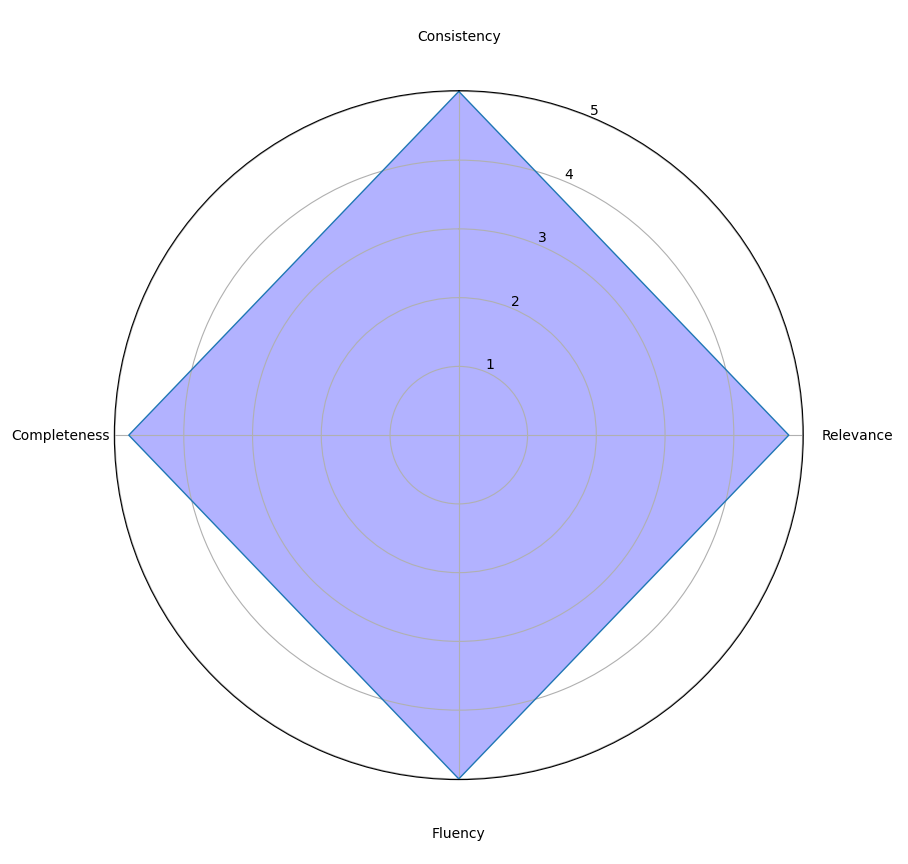
\includegraphics[width=\textwidth]{images/radar.png} 
  \caption{Evaluation results for prototype version of the GNA QA system.}
  \label{fig:proto_results}
\end{figure}


\section{Retrieval Performance and Ablation Studies}\label{sec:retrieval_ablation}
Retrieval performance pertinent to the full-scale system implementation was benchmarked in the experimental setup across different strategies: Dense, BM25, and Hybrid variants, with optional query rewriting and cross-encoder reranking. All runs were evaluated with @5 cut-offs -- R@5, MRR, nDCG@5, AP@5 --, complemented by latency measurements (seconds per query). This setup enables a consistent comparison of coverage, ranking quality, and efficiency across methods. The benchmarked retrieval scores and the different configurations tested are summarised in \autoref{tab:benchmark}.\\

\noindent The findings highlight distinct trade-offs across retrieval methods, presented hereafter.\\

\noindent \textbf{Single-hop dataset.}\\
The best overall performance was achieved by the \textbf{Hybrid + Score-blend} method without query rewriting and reranking (R@5 = 70.27, MRR = 48.59, nDCG@5 = 54.02, AP@5 = 48.59), with latency around 0.55s. This configuration consistently outperformed \textbf{Dense} retriever -- the system’s initial baseline -- and \textbf{BM25} alone, showing the benefits of combining lexical and semantic signals. A close second was \textbf{Hybrid + Weighted RRF} (R@5 = 69.68, nDCG@5 = 52.49) at slightly lower latency (0.33s).
\textbf{BM25} without extras proved a strong efficiency (R@5 = 65.15) and remained by far the fastest method ($\approx$ 0.001s), though it lagged behind hybrids in ranking quality. \textbf{Dense} retrieval showed competitive early-rank placement (MRR = 47.04) but lower recall and nDCG, confirming its limits when used in isolation.\\

\noindent \textbf{Combined (single-hop + multi-hop).}\\
Here, absolute scores dropped due to the increased complexity of multi-hop queries and the @5 cutoff, but the relative ordering of methods remained stable. \textbf{Hybrid + Score-blend} again provided the best balance, with R@5 = 55.35 and AP@5 = 36.69 at 0.45s. \textbf{BM25} retained an edge in precision at early ranks (MRR = 51.23, nDCG@5 = 57.13), again with negligible latency ($\approx$ 0.001s). \textbf{Hybrid + Weighted RRF} was also competitive (R@5 = 53.98, nDCG@5 = 56.92). \textbf{Dense} retrieval remained faster than hybrids (0.19--0.82s) but less effective overall.\\

\noindent \textbf{Effect of rewriting and reranking.}\\
Across all methods, adding query rewriting or reranking consistently reduced effectiveness and inflated latency. Reranking with the MS-MARCO English cross-encoder reordered Italian, domain-specific candidates suboptimally, while rewriting perturbed terminology that BM25 depends on. In practice, this meant added latency (up to 10 s in BM25 with rerank) and systematically lower recall and precision.\\

\noindent \textbf{Latency and quality trade-offs.}\\
The experiments exposed striking interplays between latency and retrieval quality across the methods evaluated. The fastest approach was \textbf{BM25} without any additional components, achieving near-instantaneous response times of approximately 0.001 seconds.\footnote{While BM25 was also tested in isolation within these experiments, it is important to note that this method is not intended to serve as a standalone retrieval strategy in a RAG pipeline. BM25 is a purely lexical approach that operates over inverted indexes and does not support vector search in a vector database. Its role in modern RAG chains is typically complementary, improving precision through the combination of keyword-based and embedding-based retrieval methods in hybrid search. Thus, its inclusion here serves primarily as an IR benchmark rather than as a practical candidate for deployment on its own.} However, this speed came at the expense of lower recall and ranking effectiveness compared to more advanced methods. A more balanced option was provided by the \textbf{Hybrid + Score-blend} method without extras, which delivered a strong combination of recall and ranking quality while maintaining subsecond latency in the range of 0.45--0.55 seconds. This makes it particularly suitable for interactive use cases where both efficiency and retrieval accuracy are critical. In contrast, the use of \textbf{query rewriting} and \textbf{reranking} introduced substantial computational overhead, adding several seconds of latency. Crucially, these integrations did not yield meaningful improvements in retrieval quality, making them the least cost-effective option.\\

\noindent Overall, the findings suggest that hybrid methods offer the best compromise between quality and efficiency, whereas query rewriting and reranking may not justify their latency cost in practical deployments.


\begin{table}[H]
\centering
\resizebox{\linewidth}{!}{%
\setlength{\tabcolsep}{3pt}
\footnotesize
\begin{tabular}{l c c *{10}{c}} % Method, Query rewrite, Rerank, then 10 numeric columns
\toprule
& & & \multicolumn{5}{c}{\textbf{SINGLE-HOP}} & \multicolumn{5}{c}{\textbf{COMBINED (single+multi-hop)}} \\
\cmidrule(lr){4-8}\cmidrule(lr){9-13}
\textbf{Method} & \shortstack[c]{\textbf{Query}\\\textbf{rewrite}} & \textbf{Rerank} & R@5 & MRR & nDCG@5 & AP@5 & Latency & R@5 & MRR & nDCG@5 & AP@5 & Latency \\
\midrule
Dense   &  \xmark     & \xmark & 67.51 & \underline{47.04} & 52.18 & \underline{47.04} & \underline{0.29}  & 50.78 & 48.21 & 53.70 & 34.98 & \underline{0.19} \\
        &  \checkmark & \xmark & 58.07 & 36.76 & 42.09 & 36.76 & 5.98 & 42.64 & 35.41 & 41.32 & 26.24 & 3.10   \\
        & \xmark      &  \checkmark  & 45.47 & 25.41 & 30.36 & 25.41 & 1.30  & 34.57 & 27.71 & 32.90 & 19.48 & 0.82 \\
        & \checkmark  &  \checkmark  & 52.55 & 31.66 & 36.87 & 31.66 & 4.76 & 38.16 & 30.45 & 36.0 & 22.51 & 3.46     \\
\addlinespace
BM25                          & \xmark & \xmark & 65.15 & 43.56 & 48.98 & 43.56 & \textbf{0.001} & 53.09 & \textbf{51.23} & \textbf{57.13} & 35.50 & \textbf{0.001} \\
                              & \checkmark & \xmark & 57.87 & 37.37 & 42.50 & 37.37 & 1.98 & 46.65 & 42.15 & 48.33 & 29.38 & 1.20     \\
                              & \xmark      &  \checkmark  & 45.47 & 25.41 & 30.36 & 25.41 & 1.30  & 34.57 & 27.71 & 32.90 & 19.48 & 0.82 \\
                              & \checkmark  &  \checkmark  & 43.89 & 25.87 & 30.35 & 25.87 & 10.02 & 35.18 & 30.33 & 35.68 & 20.59 & 4.96     \\
Hybrid                        &          &  &  &  &  &  &  &  &  &  &  &      \\
\hspace{0.5em}\textit{+ Weighted RRF}          & \xmark   & \xmark & \underline{69.68} & 46.72 & \underline{52.49} & 46.72 & 0.33  & \textbf{53.98} & \underline{50.93} & \underline{56.92} & \underline{36.15} & 0.32 \\
                              & \checkmark & \xmark & 57.48 & 37.48 & 42.48 & 37.48 & 4.38  & 43.52 & 38.41 & 44.10 & 27.68 & 3.21     \\
                              & \xmark      &  \checkmark  & 43.50 & 24.70 & 29.33 & 24.70 & 1.67  & 33.06 & 26.36 & 31.26 & 18.70 & 0.87 \\
                              & \checkmark  &  \checkmark  & 38.58 & 21.14 & 25.47 & 21.14 & 6.51 & 29.98 & 23.95 & 28.66 & 16.44 & 6.75     \\
\addlinespace
\hspace{0.5em}\textit{+ Score-blend}   & \xmark   & \xmark & \textbf{70.27} & \textbf{48.59} & \textbf{54.02} & \textbf{48.59} & 0.55 & \underline{53.35} & 50.84 & 56.48 & \textbf{36.69} & 0.45     \\
                              & \checkmark & \xmark & 57.67 & 37.17 & 42.31 & 37.17 & 4.57 & 43.61 & 38.16 & 43.87 & 27.52 & 3.99   \\
                              & \xmark      &  \checkmark  & 43.70 & 24.89 & 29.53 & 24.89 & 2.64 & 33.14 & 26.21 & 31.14 & 18.70 & 1.22   \\
                              & \checkmark  &  \checkmark  & 38.58 & 21.47 & 25.72 & 21.47 & 6.44 & 30.13 & 23.98 & 28.82 & 16.55 & 4.8   \\
\bottomrule
\end{tabular}%
}
\caption{Results for different retrieval methods on the test datasets. Best per column is bold and the second-best is underlined. Latency is measured in seconds per query. Reranking is performed using the \textit{cross-encoder/ms-marco-MiniLM-L-6-v2} model.}
\label{tab:benchmark}
\end{table}


\section{Qualitative Analysis}
The re-engineered system was evaluated not only through intrinsic metrics but also via direct user feedback, providing a complementary perspective on performance. As shown in \autoref{fig:ratings_}, user ratings distributed as follows: 65\% of answers received 3 stars (``Good''), 25\% received 2 stars (``Fair''), and 10\% received 1 star (``Poor'').


\begin{figure}[H]
  \centering
  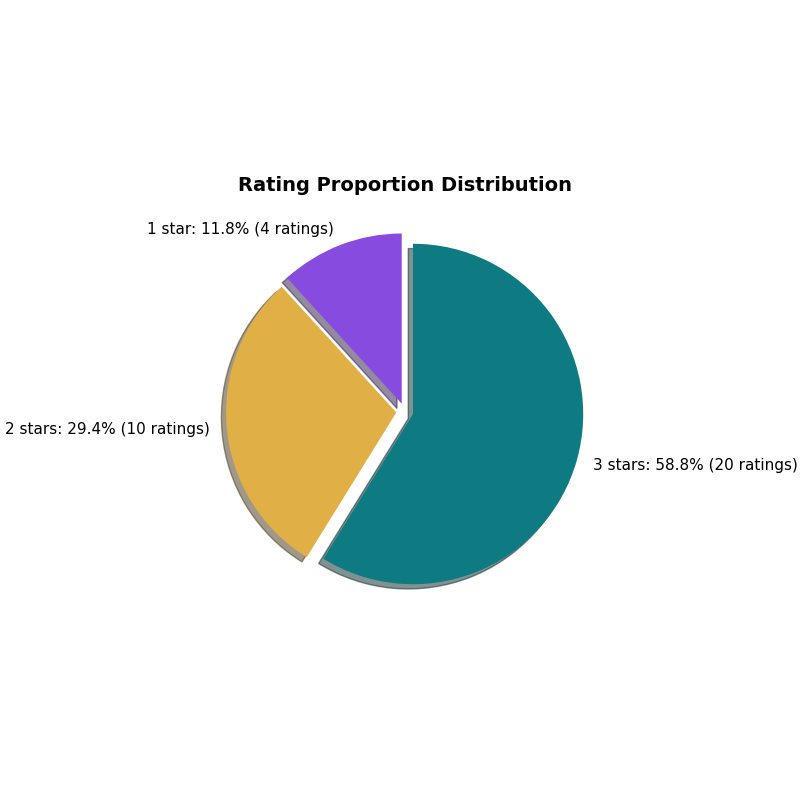
\includegraphics[width=\textwidth]{images/rating_proportions.png} 
  \caption{Distribution of user feedback ratings, showing the proportion of responses evaluated as poor (1 star), fair (2 stars), and good (3 stars).}
  \label{fig:ratings_}
\end{figure}

Instances of lower relevance were generally linked to ambiguous queries or to cases where vector sparsity limited the number of retrieved chunks. Despite these shortcomings, users highlighted several strengths: the system’s multilingual capabilities, the user-friendly interface, and the attempt to provide traceability through citations -- though, as discussed in \autoref{chap:discussion}, the citation mechanism requires further refinement.

Edge-case testing yielded additional insights. For out-of-domain queries, the system largely succeeded in avoiding hallucinations by producing cautious fallback responses. For example, (\autoref{fig:edge-case}), illustrates a query about contemporary art exhibitions in Rome: although the reply is incomplete and does not provide relevant content to the query, it faithfully reflects the system prompt’s instruction to refrain from answering questions outside the GNA scope, instead redirecting the user to the knowledge base.

Equally instructive were the tests on HTML snippets retrieval -- a particular feature of the GNA user manual where HTML tags are embedded as procedural instructions for the formatting of QGIS layouts. In these cases, the assistant correctly surfaced and rendered the relevant ``code'' blocks (see \autoref{fig:edge-case_code}), preserving both syntax and explanatory context. This demonstrated the system’s capacity to handle heterogeneous content types aside from plain text, thus addressing one of the distinctive characteristics of the GNA documentation.\\

\noindent Overall, the feedback evaluation confirmed the capability and added value of a RAG pipeline tailored to the GNA corpus. The prototype established proof of concept, while the full-scale implementation improved retrieval robustness and scalability. Although some challenges persist -- particularly with completeness, citation reliability, and response latency under query rewriting and reranking -- the system consistently produced relevant, fluent, and context-aware answers, confirming its potential as a practical assistant for navigating the GNA documentation.

\vspace{0.5em}
\begin{figure}[H]
  \centering
  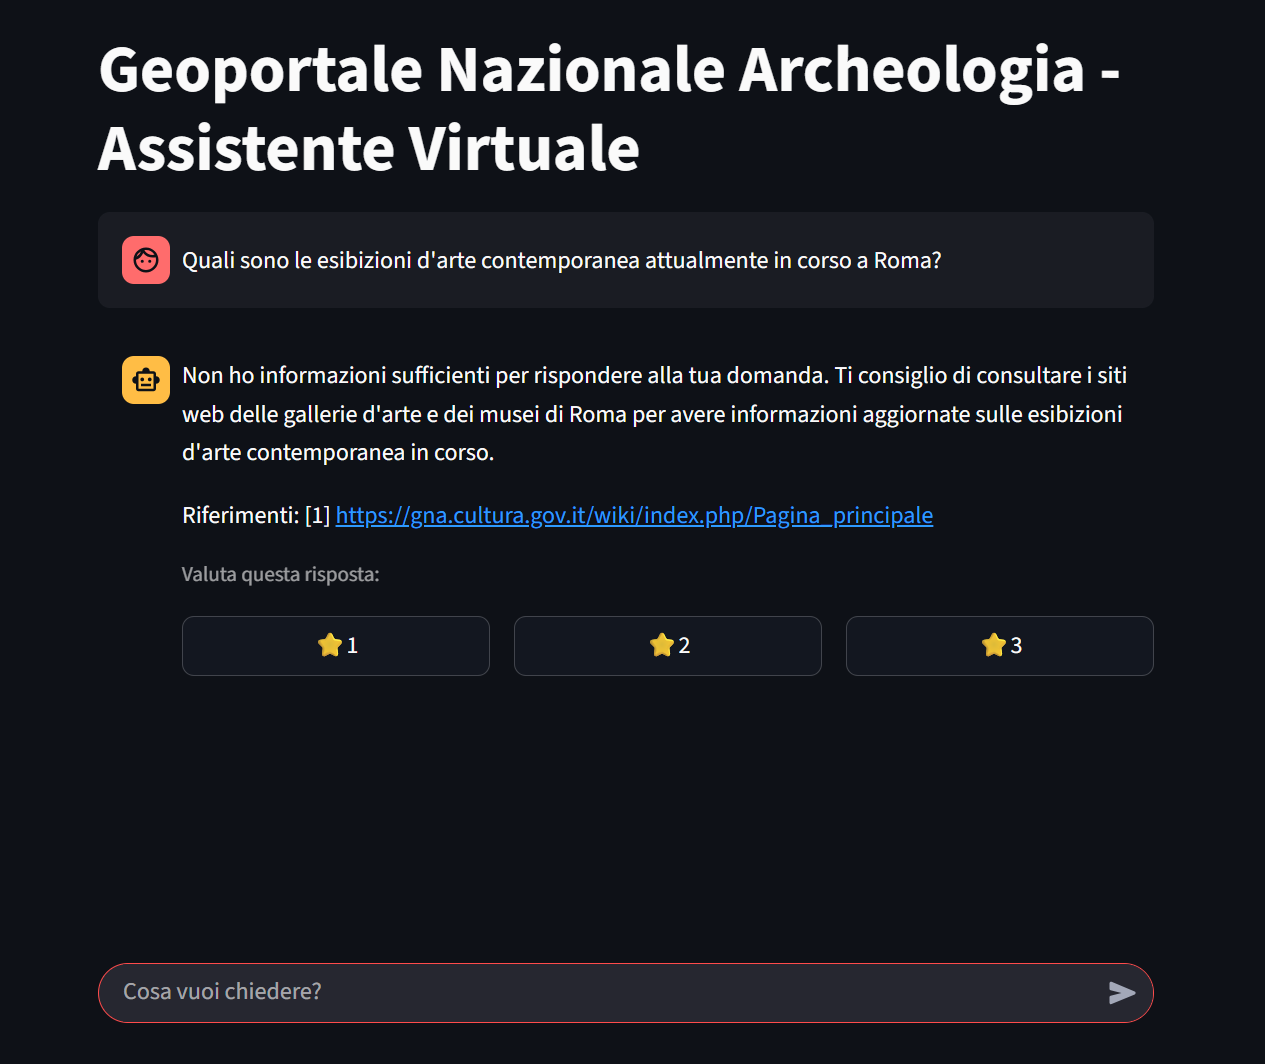
\includegraphics[width=\textwidth]{images/edge_case_response.png} 
  \caption{Edge case test of the GNA AI Assistant, showing an out-of-domain query about contemporary art exhibitions in Rome and the system’s fallback response with redirection to the GNA knowledge base.}
  \label{fig:edge-case}
\end{figure}

\begin{figure}[H]
  \centering
  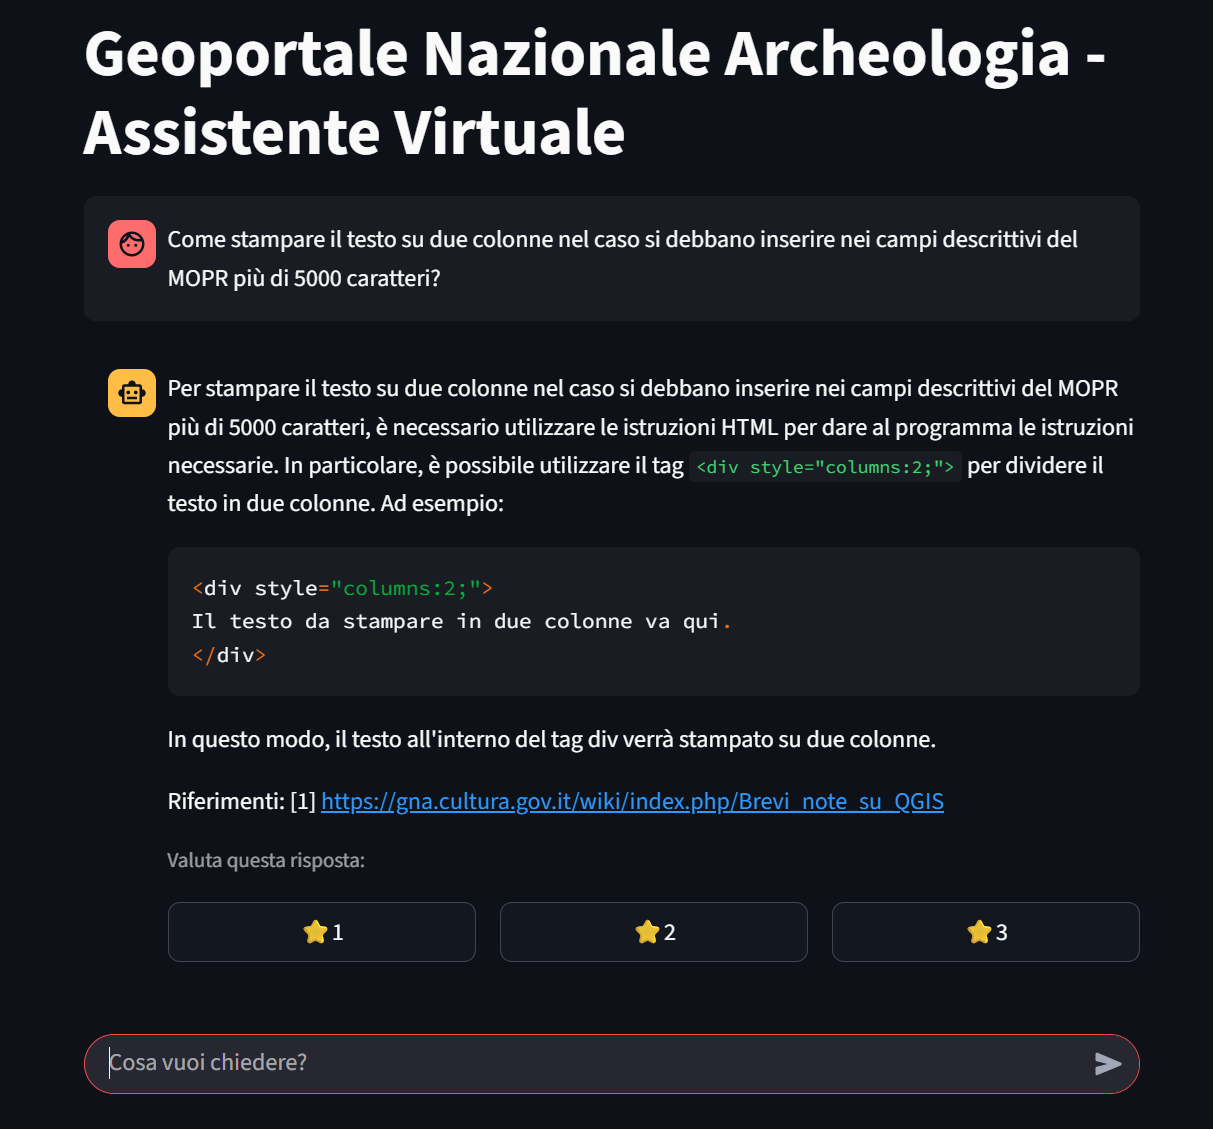
\includegraphics[width=\textwidth]{images/risposta_assistente_con_codice.png} 
  \caption{Example of the GNA QA system retrieving and presenting HTML code snippets from the knowledge base.}
  \label{fig:edge-case_code}
\end{figure}


\end{spacing}
\chapter{Discussion}
\label{chap:discussion}
\pdfcomment{WIP}
\begin{spacing}{1.5}

\section{Further Development}

specializzazione sul dominio archeologia

\end{spacing}
\chapter{Conclusion}
\label{chap:conclusion}
\begin{spacing}{1.5}
This thesis has presented the design, implementation, and evaluation of an end-to-end question-answering system for the \textit{Geoportale Nazionale Archeologia (GNA)} \citep{gna_wiki_2024}, showing how retrieval-augmented generation (RAG) can be applied to improve access to highly specialised cultural heritage documentation. While developed for a specific institutional use case, the GNA AI assistant offers insights of broader relevance -- both technical and scholarly -- into the evolving role of AI within the digital humanities.

The contributions are threefold. First, the system itself: a functioning assistant powered by AI, that systematically integrates crawling, chunking, semantic embedding, retrieval, generation, and feedback into a coherent architecture, tested across synthetic test datasets and live user interactions. Second, the evaluation framework: a dual approach that combined intrinsic retrieval metrics with human-centred assessments, making visible both capability at system level and performance as experienced by end users. Third, the methodological reflections: an exploration of the trade-offs -- between precision and recall, fluency and completeness, speed and accuracy -- that define the practical life of RAG systems in real-world contexts.

The results confirm that RAG can enhance access to dense archaeological resources, producing responses with a swifter and more accessible character than the laborious manual consultation of numerous technical records. At the same time, they underscore the fragility of such systems. Performance proves highly sensitive to corpus structure, domain vocabulary, and infrastructural constraints -- factors that remain crucial yet challenging to sustain -- and evaluation practices, when based on synthetic data, risk diverging from the texture of real user needs. The GNA QA system should therefore not be mistaken for a surrogate of scholarly interpretation. Its contribution is more modest but also more practical: it acts as an intermediary agent between users and documents, disclosing relevant passages, clarifying information flows, and enabling quicker orientation within complex materials.

Looking ahead, several fronts stand out for further development:
\begin{itemize}
    \item Technical refinements will be required. In particular, retrieval recall, especially for multi-hop queries, must be improved through higher candidate thresholds or repacking strategies. Provenance mechanisms need stabilisation, so that citations become reliable and trust is reinforced. 
    \item Long-term adaptability must be addressed, with strategies for updating embeddings as the knowledge base evolves and for handling security and privacy more explicitly.
    \item Evaluation must move toward more consistent collaboration with archaeologists and cultural heritage professionals, ensuring that system performance is judged not only by technical metrics but also by disciplinary relevance.
\end{itemize}

These improvements will be essential if RAG systems are to move from prototypes into robust infrastructures within the cultural heritage sector. However, what matters most here reaches beyond technical optimisation, as the contribution of this project aims at heading further than incremental adjustments. 

This work shows how the design of AI systems, whether in cultural heritage or other domains, is shaped by the intersection of methodological choices, infrastructural realities, and ethical considerations. From this perspective, the integration of RAG into heritage infrastructures is not merely a technical upgrade, but a reconfiguration of how knowledge is accessed, contextualised, and mediated. Archaeology, with its dispersed and stratified documentation, offers a particularly vivid test case: here, RAG has the capacity to weave fragmented records into coherent accounts oriented around user queries. Yet such promise is inseparable from risk -- the risk of oversimplification, of introducing artificial coherence, of hallucination. For this reason, critical human oversight remains indispensable, ensuring that these tools serve as mediators rather than substitutes in the interpretation of cultural knowledge. 

And still, the outlook remains fundamentally hopeful. Even amid these methodological challenges, AI-driven tools demonstrate real potential to expand access to cultural heritage resources. Their significance is not confined to technical infrastructure, but extends to the cultural and intellectual domains they touch. By presenting both the achievements and the limitations encountered along the way with transparency, this thesis seeks to contribute to the ongoing dialogue between AI and the humanities, offering a vision of AI’s evolving role as a catalyst for new forms of stewardship, interpretation, and engagement with cultural heritage.

Future research should extend this orbit, setting new vectors toward the multitude of possible directions, each illuminating a different constellation of inquiry. One promising outlet is multimodal retrieval, where text, images, and geospatial data are brought together within unified pipelines. Another is the development of models adapted to specific domains, multilingual in scope and capable of reflecting the linguistic and cultural diversity of heritage data. Equally important are collaborative evaluation frameworks that integrate field's experts into the assessment process, producing annotated datasets and conducting systematic user studies that better capture real information needs.

The scope of applications, too, could broaden considerably. From integration within GLAM realities and DSEs, to comparative studies with traditional cataloguing practices and educational settings, exploring such scenarios would provide a fuller sense of the scalability and adaptability of RAG systems across heterogeneous cultural contexts. In the specific case of digital scholarly editions, RAG might open new avenues for engaging with complex editorial data: users could, for instance, query textual variants, access synthesized accounts of critical notes, or navigate apparatus structures with greater efficiency and contextual awareness. When applied to TEI-encoded corpora, these systems might operate at a fine level of granularity -- sections, annotations, or witness readings -- while still producing responses that are coherent and transparently cited. Seen from this perspective, RAG may gradually shift from a generic AI technique toward a specialised scholarly instrument, capable of enhancing access while remaining attentive to the rigor and interpretive care central to editorial practices.

At a more conceptual level, this work opens up pressing questions. Can provenance be safeguarded without undermining usability? How can retrieval-generation pipelines scale without collapsing under their own complexity? In what ways might synthetic evaluation protocols be refined to better approximate the often messy and unpredictable demands of real-world information needs? And, perhaps most crucially, how might AI systems be designed not to replace but to complement, extend and reinforce the interpretive practices that remain at the very heart of humanistic inquiry?

The GNA AI assistant does not resolve these questions, but it makes them tangible. It shows that generative AI, when grounded in contextual retrieval, can serve as a pragmatic partner in the stewardship of cultural heritage, expanding access while respecting the epistemic specificities of the domain. More broadly, it illustrates a path forward in which AI functions less as a substitute for human understanding and more as a companion -- one that structures access, enhances discoverability, and supports informed engagement with complex resources.

In this sense, the project is less an endpoint than an invitation -- a doorway toward new questions, opportunities, and directions for future research. It offers a modest yet concrete contribution to the dialogue between generative AI and the humanities, a small brick laid in what may become a much larger hall of digital scholarship, portending toward a future in which AI technologies are not peripheral tools but structural beams within scholarly and heritage settings. The challenge now is to shape this integration with care, so that the ingenuity of technical design remains attuned to the subtleties of human knowledge. That challenge, and its possibilities, are both a weight and a promise. These will chart the course of the next explorations, where the paths of machine computation and human interpretation continue to converge, diverge, and intertwine.


\end{spacing}

\clearpage
% Appendices
\begin{appendices}
    \chapter{Implementation details}
    \label{appendix:A}

In this study, all the experiments have been performed on a system with an Intel Core i7-1185G7 CPU at 3.00 GHz, 16 GB of RAM, and integrated Intel Iris Xe Graphics with 128 MB of VRAM. 

\noindent Additionally, the following software packages have been used to implement the proposed approach: PyTorch, NumPy, Pandas, Matplotlib, SpaCy, HuggingFace...

\chapter{Abbreviations and Glossary}
\label{appendix:B}

\sloppy

\renewcommand\tabularxcolumn[1]{>{\noindent\justifying\arraybackslash}m{#1}} % justified + no indent in X columns

\footnotesize
\begin{tabularx}{\textwidth}{
  >{\raggedright\arraybackslash}p{2.5cm}
  >{\raggedright\arraybackslash}p{4cm}
  >{\noindent\justifying\arraybackslash}X
}
\caption{Abbreviations and acronyms with their full forms and definitions used in this thesis.}
\label{tab:abbreviations} \\
\\
\toprule
\textbf{Term} & \textbf{Full form} & \textbf{Glossary definition} \\
\midrule
\endfirsthead

\toprule
\textbf{Term} & \textbf{Full form} & \textbf{Glossary definition} \\
\midrule
\endhead

\midrule
\multicolumn{3}{r}{\textcolor{gray}{\emph{Continued on next page}}} \\
\endfoot

\bottomrule
\endlastfoot

AI    & Artificial intelligence & The field of computer science dedicated to creating systems capable of performing tasks that typically require human intelligence, such as reasoning, learning, and problem-solving. \\
\cmidrule(lr){1-3}
DH    & Digital humanities & An interdisciplinary field that applies computational methods and tools to humanities research, analysis, and dissemination. \\
\cmidrule(lr){1-3}
QA    & Question answering & A technology or task in which a system provides precise answers to questions posed in natural language. \\
\cmidrule(lr){1-3}
QAS   & Question-answering system & A system designed to answer questions automatically by processing natural language input, often using methods from IR and NLP. \\
\cmidrule(lr){1-3}
RAG   & Retrieval-augmented generation & An approach combining information retrieval with generative models, allowing AI to reference external data sources when generating answers. \\
\cmidrule(lr){1-3}
LLM   & Large language model & A neural network trained on massive text corpora to generate or understand human language, such as GPT or BERT. \\
\cmidrule(lr){1-3}
IR    & Information retrieval & The process of searching, retrieving, and ranking relevant documents or data from large collections based on user queries. \\
\cmidrule(lr){1-3}
GNA   & Geoportale Nazionale Archeologia & Italy's institutional repository for archaeological data, hosting extensive documentation and resources related to the country's cultural heritage. \\
\cmidrule(lr){1-3}
MiC & Ministero della Cultura & The Italian Ministry of Culture, responsible for the preservation and promotion of Italy's cultural heritage. \\
\cmidrule(lr){1-3}
MiBACT & Ministero dei Beni e delle Attività Culturali e del Turismo & The former name of the Italian Ministry of Culture, which was responsible for cultural heritage and tourism before its reorganization in 2021. \\
\cmidrule(lr){1-3}
CNR & Consiglio Nazionale delle Ricerche & The Italian National Research Council, a major public research institution that conducts scientific research across various disciplines, including cultural heritage. \\
\cmidrule(lr){1-3}
DG-Ant & Direzione Generale Archeologia, Belle Arti e Paesaggio & The Directorate General for Archaeology, Fine Arts, and Landscape within the Italian Ministry of Culture, overseeing archaeological heritage and cultural sites. \\
\cmidrule(lr){1-3}
ICA & Istituto Centrale per l’Archeologia & The Central Institute for Archaeology in Italy, established in 2016 as part of the Ministry of Culture, responsible for archaeological research and documentation. \\
\cmidrule(lr){1-3}
ICCD & Istituto Centrale per il Catalogo e la Documentazione & The Central Institute for Cataloging and Documentation, part of the Italian Ministry of Culture, responsible for cataloging cultural heritage assets and proposing best practices. \\
\cmidrule(lr){1-3}
SiGECweb &  Sistema Informativo Generale del Catalogo & A web platform that handles every stage of cultural heritage cataloguing, from standard creation and code assignment to cataloguing diverse assets and publishing records online for public access. \\
\cmidrule(lr){1-3}
GIS & Geographic information system & A computer system, including software and hardware, designed to capture, store, manipulate, analyze, manage, and present spatial or geographic data, often used in archaeology for mapping and spatial analysis. \\
\cmidrule(lr){1-3}
QGIS &  & A particular GIS software that is free and open-source. \\
\cmidrule(lr){1-3}
GLAM   & Galleries, Libraries, Archives and Museums & A collective term for institutions that preserve and provide access to cultural heritage in the public interest. \\
\cmidrule(lr){1-3}
KB    & Knowledge base & A structured collection of information or data, often used to support reasoning, search, or retrieval in AI systems. \\
\cmidrule(lr){1-3}
NLP   & Natural language processing & The area of AI focused on enabling computers to understand, interpret, and generate human language. \\
\cmidrule(lr){1-3}
NLG   & Natural language generation & The process of automatically generating human-like text from structured data or models, often used in chatbots and content creation. \\
\cmidrule(lr){1-3}
NL & Natural language & The everyday language used by humans for communication, which NLP systems aim to understand and generate. \\
\cmidrule(lr){1-3}
ML    & Machine learning & A subset of AI that involves training algorithms to recognize patterns and make decisions based on data. \\
\cmidrule(lr){1-3}
NER   & Named entity recognition & A subtask of NLP that identifies and classifies named entities (e.g., people, organizations, locations) in text. \\
\cmidrule(lr){1-3}
EL    & Entity linking & The process of connecting named entities in text to their corresponding entries in a knowledge base, enhancing understanding and retrieval. \\
\cmidrule(lr){1-3}
TF-IDF & Term Frequency-Inverse Document Frequency & A statistical measure used in IR to evaluate how important a word is to a document relative to a corpus, balancing term frequency and document rarity. \\
\cmidrule(lr){1-3}
BM25  & Best match 25 & A ranking function used in IR to estimate the relevance of documents to a given search query, based on term frequency and document length normalization.\\
\cmidrule(lr){1-3}
PRF   & Precision-Recall-F1 & Metrics used to evaluate the performance of classification models, where precision measures the accuracy of positive predictions, recall measures the ability to find all relevant instances, and F1 is the harmonic mean of precision and recall. \\
\cmidrule(lr){1-3}
RDF   & Resource Description Framework & A standard model for data interchange on the web, allowing structured representation of information about resources in a machine-readable format. \\
\cmidrule(lr){1-3}
SQL   & Structured Query Language & A standard programming language used for managing and manipulating relational databases, allowing users to query, insert, update, and delete data. \\
\cmidrule(lr){1-3}
SPARQL &  & A query language and protocol used to retrieve and manipulate data stored in Resource Description Framework (RDF) format, commonly used for querying knowledge graphs. \\
\cmidrule(lr){1-3}  
ontology &  & A formal representation of a set of concepts within a domain and the relationships between those concepts, used to enable knowledge extraction, sharing and reuse. \\
\cmidrule(lr){1-3}
JSON  & JavaScript Object Notation & A lightweight data interchange format that is easy for humans to read and write, and easy for machines to parse and generate, often used for data exchange in web applications. \\
\cmidrule(lr){1-3}
TREC  & Text REtrieval Conference & An ongoing series of workshops and evaluations focused on advancing research in text retrieval and related tasks. \\
\cmidrule(lr){1-3}
LMIR & Language model information retrieval & A method of using language models to improve the effectiveness of information retrieval systems by leveraging their understanding of language and context. \\
\cmidrule(lr){1-3}
RNN   & Recurrent Neural Network & A type of neural network architecture designed to process sequential data by maintaining a form of memory of previous inputs. \\
\cmidrule(lr){1-3}
LSTM  & Long Short-Term Memory & A special kind of RNN capable of learning long-range dependencies, often used for tasks like language modeling or time series prediction. \\
\cmidrule(lr){1-3}
CRF   & Conditional Random Field & A probabilistic graphical model used for structured prediction, especially in NLP tasks such as sequence labeling. \\
\cmidrule(lr){1-3}
SVM   & Support Vector Machine & A supervised machine learning algorithm used for classification and regression, which finds the optimal boundary between classes in the feature space. \\
\cmidrule(lr){1-3}
Word2Vec & Word to Vector & A technique for representing words as vectors in a continuous vector space, capturing semantic relationships between words based on their context in large text corpora. \\
\cmidrule(lr){1-3}
GloVe  & Global Vectors for Word Representation & An unsupervised learning algorithm for obtaining vector representations of words, which captures global statistical information from a corpus. \\
\cmidrule(lr){1-3}
BERT  & Bidirectional Encoder Representations from Transformers & A pre-trained language model that uses the Transformer architecture to understand the context of words in a sentence by considering both left and right contexts simultaneously. \\
\cmidrule(lr){1-3}
GPT   & Generative pre-trained Transformer & A type of LLM that uses the Transformer architecture.\\
\cmidrule(lr){1-3}
T5    & Text-to-Text Transfer Transformer & A versatile LLM that treats all NLP tasks as text-to-text problems, allowing it to be fine-tuned for various applications. \\
\cmidrule(lr){1-3}
E5    & Embedding-based model for information retrieval & A family of models designed to generate high-quality embeddings for text, improving retrieval performance in IR tasks. \\
\cmidrule(lr){1-3}
BGE   & BAAI general embedding & A family of models designed to generate high-quality embeddings for text, improving retrieval performance in IR tasks. \\
\cmidrule(lr){1-3}
intfloat & intfloat/e5 & A specific implementation of the E5 model, optimized for generating embeddings for information retrieval tasks. \\
\cmidrule(lr){1-3}
LLM-embedder &   & A model designed to generate embeddings for text using large language models, enhancing the quality of semantic representations for retrieval tasks. \\
\cmidrule(lr){1-3}
embeddings &    & Dense vector representations of text that capture semantic meaning, used in various NLP tasks including retrieval and classification. \\
\cmidrule(lr){1-3}
chunking &    & The process of breaking down text into smaller, manageable pieces or ``chunks'' to facilitate processing and analysis in NLP tasks. \\
\cmidrule(lr){1-3}
vector database &    & A specialized database designed to store and retrieve high-dimensional vectors efficiently, often used in RAG systems for managing embeddings. \\
\cmidrule(lr){1-3}
retriever &    & A component of a system responsible for searching and retrieving relevant documents or information from a database or corpus based on user queries. \\
\cmidrule(lr){1-3}
ranking function &    & A mathematical function used to score and order documents based on their relevance to a given query, often employed in IR systems. \\
\cmidrule(lr){1-3}
XML & eXtensible Markup Language & A markup language used to encode documents in a format that is both human-readable and machine-readable, often used for data interchange. \\
\cmidrule(lr){1-3}
TEI & Text Encoding Initiative & A set of guidelines for encoding literary and linguistic texts in XML, providing a standardized way to represent complex textual structures. \\
\cmidrule(lr){1-3} 
MARC/RDA & Machine-Readable Cataloging / Resource Description and Access & Standards for encoding bibliographic information in a machine-readable format, widely used in libraries and information systems. \\
\cmidrule(lr){1-3}
GROBID & GeneRation Of BIbliographic Data & A machine learning library for extracting and structuring bibliographic information from scholarly documents, often used in academic publishing and research. \\
\cmidrule(lr){1-3}
Milvus & Milvus Vector Database & An open-source vector database designed for efficient storage, indexing, and retrieval of high-dimensional vectors, commonly used in RAG systems. \\
\cmidrule(lr){1-3}
Faiss  & Facebook AI Similarity Search & A library for efficient similarity search and clustering of
dense vectors, widely used in RAG systems for indexing and searching large datasets. \\
\cmidrule(lr){1-3}
Qdrant & Qdrant Vector Database & An open-source vector database that provides efficient storage and retrieval of high-dimensional vectors, supporting hybrid search capabilities. \\
\cmidrule(lr){1-3}
DLM reranking & Deep language model-based reranking uses fine-tuned models that jointly encode query-document pairs and classify their relevance as ``true'' or ``false''. At inference, documents are ranked by the probability of being labeled ``true''. \\
\cmidrule(lr){1-3}
HyDE  & Hybrid Document Embedding & A method that combines dense vector representations with traditional keyword-based indexing to improve retrieval performance in RAG systems. \\
\cmidrule(lr){1-3}
Hybrid Search &  & A search approach that combines vector-based retrieval with traditional keyword search, allowing for more comprehensive and context-aware results in RAG systems. \\
\cmidrule(lr){1-3}
TILDE &  & A framework designed to facilitate the development and deployment of RAG systems, providing tools for data preparation, indexing, and retrieval. \\
\cmidrule(lr){1-3}
TILDEv2 &  & An updated version of the TILDE framework, incorporating improvements in efficiency and performance. \\
\cmidrule(lr){1-3}
LTR   & Learning-to-Rank & A machine learning approach used to optimize the ranking of search results based on user interactions and relevance feedback, improving the quality of retrieved documents in RAG systems. \\
\cmidrule(lr){1-3}
Self-RAG & Self-Retrieval-Augmented Generation & A variant of RAG where the system retrieves relevant information from its own generated content, enhancing the context and accuracy of responses. \\
\cmidrule(lr){1-3}
RAGAS & Retrieval-Augmented Generation with Adaptive Sampling & An advanced RAG approach that dynamically selects and retrieves the most relevant information based on the context of the query, improving the efficiency and accuracy of responses. \\
\cmidrule(lr){1-3}
XAI & Explainable Artificial Intelligence & A field of AI focused on rendering the decision-making processes of AI systems transparent and understandable to humans, often used to build trust and accountability in AI applications. \\
\cmidrule(lr){1-3}
RAG-Chain & Retrieval-Augmented Generation Chain & A method that links multiple RAG components in a sequence. \\
\cmidrule(lr){1-3}
ArCo & Italian Cultural Heritage knowledge graph & A knowledge graph representing Italian cultural heritage, providing structured information about historical sites, artifacts, and related entities. \\
\bottomrule
\end{tabularx}



\end{appendices}


\chapter*{Acknowledgments}
\addcontentsline{toc}{chapter}{Acknowledgments}
\clearpage
\sloppy
% Back Matter
\backmatter
\pagestyle{fancy}

\phantomsection
\addcontentsline{toc}{chapter}{Bibliography}
\printbibliography

\end{document}